%Este trabalho está licenciado sob a Licença Atribuição-CompartilhaIgual 4.0 Internacional Creative Commons. Para visualizar uma cópia desta licença, visite http://creativecommons.org/licenses/by-sa/4.0/deed.pt_BR ou mande uma carta para Creative Commons, PO Box 1866, Mountain View, CA 94042, USA.

\documentclass[12pt]{book}

\input ../preambulo.tex

\makeindex

\begin{document}

\ifispython
\lstset { %
  language=Python,
  numbers=left,
  numberstyle=\small,
  stepnumber=1,    
  firstnumber=1,
  numberfirstline=true,
  extendedchars=true,
  inputencoding=utf8,
  upquote=true,
  basicstyle=\ttfamily,
  keywordstyle=\ttfamily,
  stringstyle=\ttfamily,
  commentstyle=\ttfamily,
  showspaces=false,
  showstringspaces=false,
  showtabs=false
}
\fi


\frontmatter

\title{Geometria Analítica}
\author{Pedro H A Konzen}
\date{\today}
\ifishtml
\else
\addcontentsline{toc}{chapter}{Capa}
\fi

\maketitle

%Este trabalho está licenciado sob a Licença Atribuição-CompartilhaIgual 4.0 Internacional Creative Commons. Para visualizar uma cópia desta licença, visite http://creativecommons.org/licenses/by-sa/4.0/ ou mande uma carta para Creative Commons, PO Box 1866, Mountain View, CA 94042, USA.

\chapter*{Licença}\label{licenca}
\addcontentsline{toc}{chapter}{Licença}

Este trabalho está licenciado sob a Licença Atribuição-CompartilhaIgual 4.0 Internacional Creative Commons. Para visualizar uma cópia desta licença, visite http://creativecommons.org/licenses/by-sa/4.0/deed.pt\_BR ou mande uma carta para Creative Commons, PO Box 1866, Mountain View, CA 94042, USA.

%Este trabalho está licenciado sob a Licença Atribuição-CompartilhaIgual 4.0 Internacional Creative Commons. Para visualizar uma cópia desta licença, visite http://creativecommons.org/licenses/by-sa/4.0/deed.pt_BR ou mande uma carta para Creative Commons, PO Box 1866, Mountain View, CA 94042, USA.

\chapter*{Prefácio}\label{prefacio}
\addcontentsline{toc}{chapter}{Prefácio}

O site \href{https://www.notaspedrok.com.br}{notaspedrok.com.br} é uma plataforma que construí para o compartilhamento de minhas notas de aula. Essas anotações feitas como preparação de aulas é uma prática comum de professoras/es. Muitas vezes feitas a rabiscos em rascunhos com validade tão curta quanto o momento em que são concebidas, outras vezes, com capricho de um diário guardado a sete chaves. Notas de aula também são feitas por estudantes - são anotações, fotos, prints, entre outras formas de registros de partes dessas mesmas aulas. Essa dispersão de material didático sempre me intrigou e foi o que me motivou a iniciar o site.

Com início em 2018, o site contava com apenas três notas incipientes. De lá para cá, conforme fui expandido e revisando os materais, o site foi ganhando acessos de vários locais do mundo, em especial, de países de língua portugusa. No momento, conta com 13 notas de aula, além de minicursos e uma coleção de vídeos e áudios.

As notas de \emph{Redes Neurais Artificiais} fazem uma introdução às redes neuraus artificiais com enfase na resolução de problemas de matemática. Como ferramenta de apoio computacional, códigos exemplos são trabalhos em linguagem {\python}, mais especificamente, com o pacote de aprendizagem de máquina {\pytorch}.

Aproveito para agradecer a todas/os que de forma assídua ou esporádica contribuem com correções, sugestões e críticas! ;)

\begin{flushright}
  Pedro H A Konzen

  \url{https://www.notaspedrok.com.br}
\end{flushright}



\tableofcontents
\addcontentsline{toc}{chapter}{Sumário}

\mainmatter

%Este trabalho está licenciado sob a Licença Atribuição-CompartilhaIgual 4.0 Internacional Creative Commons. Para visualizar uma cópia desta licença, visite http://creativecommons.org/licenses/by-sa/4.0/deed.pt_BR ou mande uma carta para Creative Commons, PO Box 1866, Mountain View, CA 94042, USA.

\chapter{Sistema de coordenadas}\label{cap_scoord}
\thispagestyle{fancy}

A geometria analítica é uma área interdisciplinar da matermática que faz o estudo de objetos da geometria através de estruturas algébricas (equações e inequações algébricas). Para tanto, o primeiro passo é a construção (definição) de um sistema de coordenadas, no qual os objetos geométricos serão referenciados.

\section{Sistema de coordenadas no espaço}\label{cap_scoord_sec_scoord}

Um sistema de coordenadas no espaço (euclidiano) é constituído de um ponto $O$ e uma base de vetores $B = (\vec{e}_1, \vec{e}_2, \vec{e}_3)$ no espaço. Dado um tal sistema, temos que cada ponto $P$ determina de forma única um vetor $\overrightarrow{OP} = (x,y,z)$ e vice-versa. Assim sendo, definimos que o ponto $P$ tem coordenadas $(x,y,z)$. Veja a figura abaixo.

\begin{figure}[H]
  \centering
  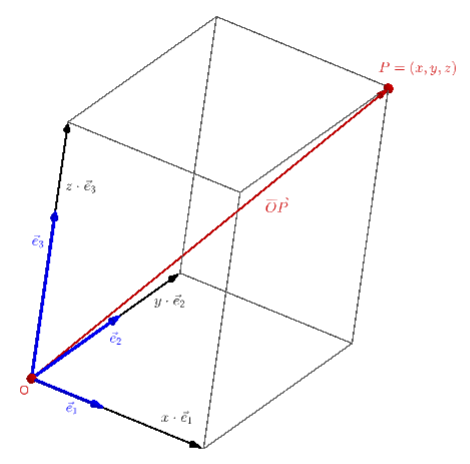
\includegraphics[width=0.8\textwidth]{cap_scoord/dados/fig_scoord/fig}
  \caption{Ilustração de um sistema de coordenadas no espaço.}
  \label{fig:scoord}
\end{figure}

O ponto $O$ é chamado de \emph{origem} (do sistema de coordenadas) e tem coordenadas $O=(0,0,0)$. Dado um ponto $P=(x,y,z)$, chama-se $x$ de sua \emph{abscissa}, $y$ de sua \emph{ordenada} e $z$ de sua \emph{cota}. As retas que passam por $O$ e têm, respectivamente, as mesmas direções de $\vec{e}_1$, $\vec{e}_2$ e $\vec{e}_3$ são chamadas de \emph{eixo das abscissas}, \emph{eixo das ordenadas} e \emph{eixo das cotas}. Os planos que contém $O$ e representantes de dois vetores da base $B$ são chamados de \emph{planos coordenados}.

\begin{figure}[H]
  \centering
  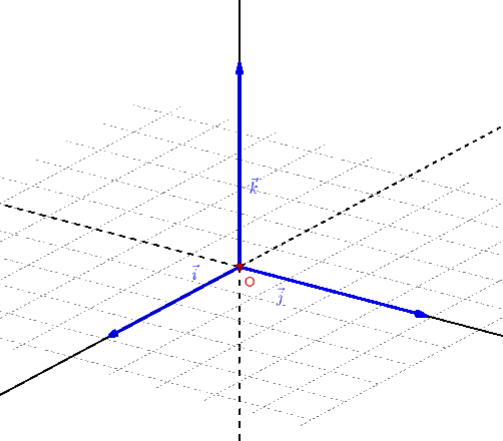
\includegraphics[width=0.7\textwidth]{./cap_scoord/dados/fig_sis_coord_orto/fig}
  \caption{Ilustração de um sistema de coordenadas ortonormal.}
  \label{fig:sis_coord_orto}
\end{figure}

Salvo explicitado ao contrário, trabalharemos com um \emph{sistema de coordenadas ortonormal}, i.e. sistema cuja base $B = (\vec{i},\vec{j},\vec{k})$ seja ortonormal. Mais ainda, estaremos assumindo que a base é positiva. Veja a Figura \ref{fig:sis_coord_orto}.

\begin{obs}\normalfont{(Relação entre pontos e vetores)}
  Seja dado um vetor $\overrightarrow{AB}$. Sabendo as coordenadas dos pontos $A = (x_A,y_A,z_A)$ e $B = (x_B,y_B,z_B)$, temos que as coordenadas do vetor $\overrightarrow{AB}$ são:
  \begin{align}
    \overrightarrow{AB} &= \overrightarrow{AO} + \overrightarrow{OB}\\
                        &= -\overrightarrow{OA} + \overrightarrow{OB}\\
                        &= -(x_A,y_A,z_A)+(x_B,y_B,z_B)\\
                        &= (x_B-x_A,y_B-y_A,z_B-z_A).
  \end{align}
  Em uma linguagem menos formal, podemos dizer que as coordenadas de $\overrightarrow{AB}$ é a resultante das coordenadas do ponto final menos as coordenadas do ponto de partida. Veja a figura abaixo.

\begin{figure}[H]
  \centering
  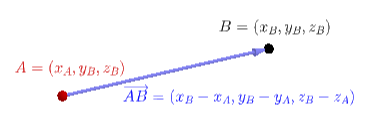
\includegraphics[width=0.6\textwidth]{./cap_scoord/dados/fig_scoord_vec_pt/fig}
  \caption{Relação entre as coordenadas dos pontos de partida e de chegada de um vetor.}
  \label{fig:scoord_vec_pt}
\end{figure}  
\end{obs}

\begin{ex}
  Dados os pontos $A = (-1,1,2)$ e $B = (3,-1,0)$, temos que o vetor $\overrightarrow{AB}$ tem coordenadas:
  \begin{equation}
    \overrightarrow{AB} = (3-(-1),-1-1,0-2) = (4,-2,-2).
  \end{equation}
\end{ex}

\begin{obs}\normalfont{(Ponto médio de um segmento)}
  Dados os pontos $A = (x_A,y_A,z_A)$ e $B = (x_B,y_B,z_B)$, podemos calcular as coordenadas do ponto médio $M = (x_M,y_M,z_M)$ do segmento $AB$. Veja a figura abaixo.

\begin{figure}[H]
  \centering
  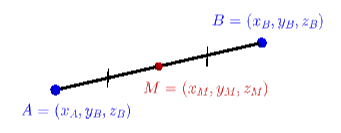
\includegraphics[width=0.6\textwidth]{./cap_scoord/dados/fig_scoord_pm/fig}
  \caption{Coordenadas do ponto médio de um segmento.}
  \label{fig:scoord_pm}
\end{figure}  

  Do fato de que $\overrightarrow{AM} = \overrightarrow{MB}$, temos
  \begin{equation}
    (x_M-x_A,y_M-y_A,z_M-z_A)=(x_B-x_M,y_B-y_M,z_B-z_M),
  \end{equation}
  Logo, segue que
  \begin{align}
    x_M-x_A &= x_B-x_M\\
    y_M-y_A &= y_B-y_M\\
    z_M-z_A &= z_B-z_M
  \end{align}
  ou, equivalentemente,
  \begin{align}
    2x_M &= x_A+x_B\\
    2y_M &= y_A+y_B\\
    2z_M &= z_A+z_B
  \end{align}
  Portanto, concluímos que
  \begin{align}
    x_M &= \frac{x_A+x_B}{2}\\
    y_M &= \frac{y_A+y_B}{2}\\
    z_M &= \frac{z_A+z_B}{2}
  \end{align}  
  Logo, temos
  \begin{equation}
  M = \left(\frac{x_A+x_B}{2},\frac{y_A+y_B}{2},\frac{z_A+z_B}{2}\right)
\end{equation}
\end{obs}

\begin{ex}
  Dados os pontos $A = (-1,1,2)$ e $B = (3,-1,0)$, temos que o ponto médio do segmento $AB$ tem coordenadas:
  \begin{align}
    M &= \left(\frac{-1+3}{2},\frac{1+(-1)}{2},\frac{2+0}{2}\right)\\
    &= (1,0,1).
  \end{align}
\end{ex}

\subsection*{Exercícios resolvidos}

\begin{exeresol}
  Sejam $A = (-1,2,1)$, $B = (1,-2,0)$ e $C = (x,2,2)$ vértices consecutivos de um triângulo isósceles, cujos lados $AC$ e $BC$ são congruentes. Determine o valor de $x$.
\end{exeresol}
\begin{resol}
  Sendo os lados $AC$ e $BC$ congruentes, temos $|\overrightarrow{AC}| = |\overrightarrow{BC}|$. As coordenadas de $\overrightarrow{AC}$ são
  \begin{equation}
    \overrightarrow{AC} = (x-(-1),2-2,2-1) = (x+1,0,1)
  \end{equation}
  e as coordenadas de $\overrightarrow{BC}$ são
  \begin{equation}
    \overrightarrow{BC} = (x-1,2-(-2),2-0) = (x-1,4,2).
  \end{equation}
  Então, temos
  \begin{align}
    |\overrightarrow{AC}| = |\overrightarrow{BC}| &\Rightarrow \sqrt{(x+1)^2+0^2+1^2} = \sqrt{(x-1)^2+4^2+2^2}\\
                                                  &\Rightarrow (x+1)^2+0^2+1^2 = (x-1)^2+4^2+2^2\\
                                                  &\Rightarrow x^2+2x+1+1 = x^2-2x+1+16+4\\
                                                  &\Rightarrow 4x = 19\\
                                                  &\Rightarrow x = \frac{19}{4}.
  \end{align}
\end{resol}

\begin{exeresol}
  Sejam $A = (-1,2,1)$, $B = (1,-2,0)$  e $M$ o ponto médio do intervalo $AB$. Determine as coordenadas do ponto $P$ de forma que $2AP = AM$.
\end{exeresol}
\begin{resol}
  As coordenadas do ponto médio são
  \begin{equation}
    M = \left(\frac{-1+1}{2},\frac{2+(-2)}{2},\frac{1+0}{2}\right) = \left(0,0,\frac{1}{2}\right).
  \end{equation}
  Agora, denotando $P = (x_P,y_P,z_P)$, temos
  \begin{align}
    2AP = AM &\Rightarrow 2(x_P-(-1),y_P-2,z_P-1) = \left(0-(-1),0-2,\frac{1}{2}-1\right)\\
             &\Rightarrow (2x_p+2,2y_P-4,2z_P-2) = \left(1,-2,-\frac{1}{2}\right).
  \end{align}
  Portanto
  \begin{align}
    & 2x_P+2 = 1 \Rightarrow x_P = -\frac{1}{2}\\
    & 2y_P-4 = -2 \Rightarrow y_P = 1\\
    & 2z_P-2 = -\frac{1}{2} \Rightarrow z_P = \frac{3}{4}.
  \end{align}
  Logo, $P = (-1/2,1,3/4)$.
\end{resol}

\subsection*{Exercícios}

\emconstrucao

\section{Equações da reta}\label{cap_ert_sec_eqsreta}

\subsection{Equação vetorial de uma reta}

Seja $r$ uma reta dada, $\vec{v}$ um vetor paralelo a $r$ e $A$ um ponto de $r$ (veja a Figura~\ref{fig:er_vet}). Assim sendo, $P$ é um ponto de $r$ se, e somente se, existe $\lambda\in\mathbb{R}$ tal que
\begin{equation}
  \overrightarrow{AP} = \lambda\vec{v}.
\end{equation}
Esta é chamada \emph{equação vetorial da reta} $r$.

\begin{figure}[H]
  \centering
  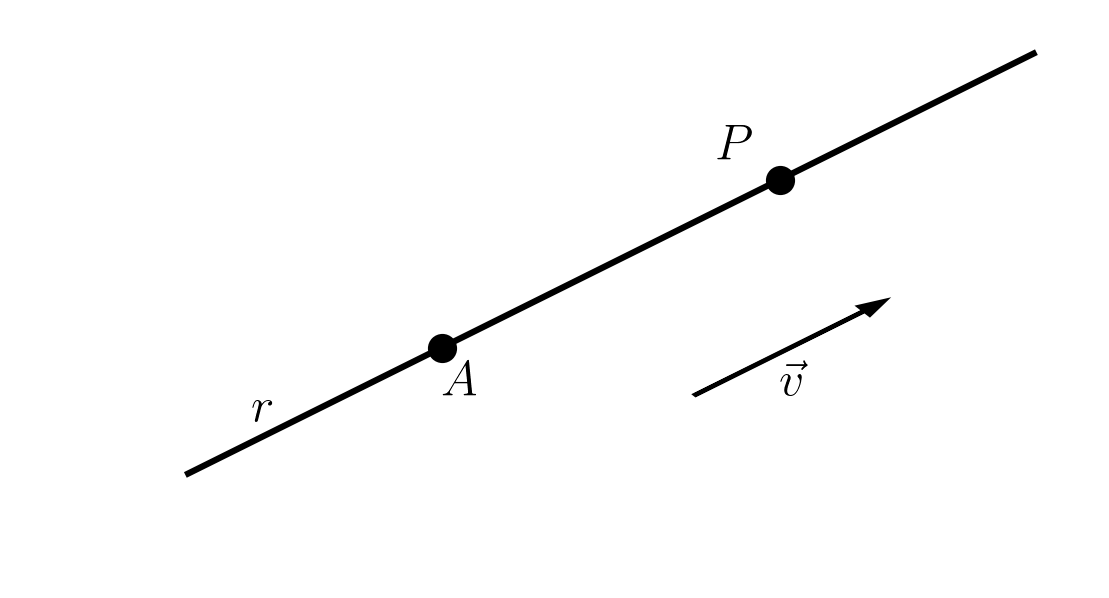
\includegraphics[width=0.5\textwidth]{./cap_er/dados/fig_er_vet/fig_er_vet}
  \caption{Equação vetorial de uma reta.}
  \label{fig:er_vet}
\end{figure}

Observe que para obtermos uma equação vetorial de uma dada reta, podemos escolher qualquer ponto $A\in r$ e qualquer vetor $\vec{v}\parallel r$, $\vec{v}\neq\vec{0}$. O vetor $\vec{v}$ escolhido é chamado de \emph{vetor diretor}.

\begin{ex}\label{ex:er_vet}
  Seja $r$ a reta que passa pelos pontos $A=(-1,-1,-2)$ e $B = (2,1,3)$ (veja a Figura \ref{fig:ex_er_vet}). O vetor
  \begin{equation}
    \vec{v} = \overrightarrow{AB} = (2-(-1),1-(-1),3-(-2)) = (3,2,5)
  \end{equation}
  é um vetor diretor de $r$. Desta forma, uma equação vetorial da reta $r$ é
  \begin{equation}
    \overrightarrow{AP} = \lambda\vec{v}.
  \end{equation}
  \begin{figure}[H]
    \centering
    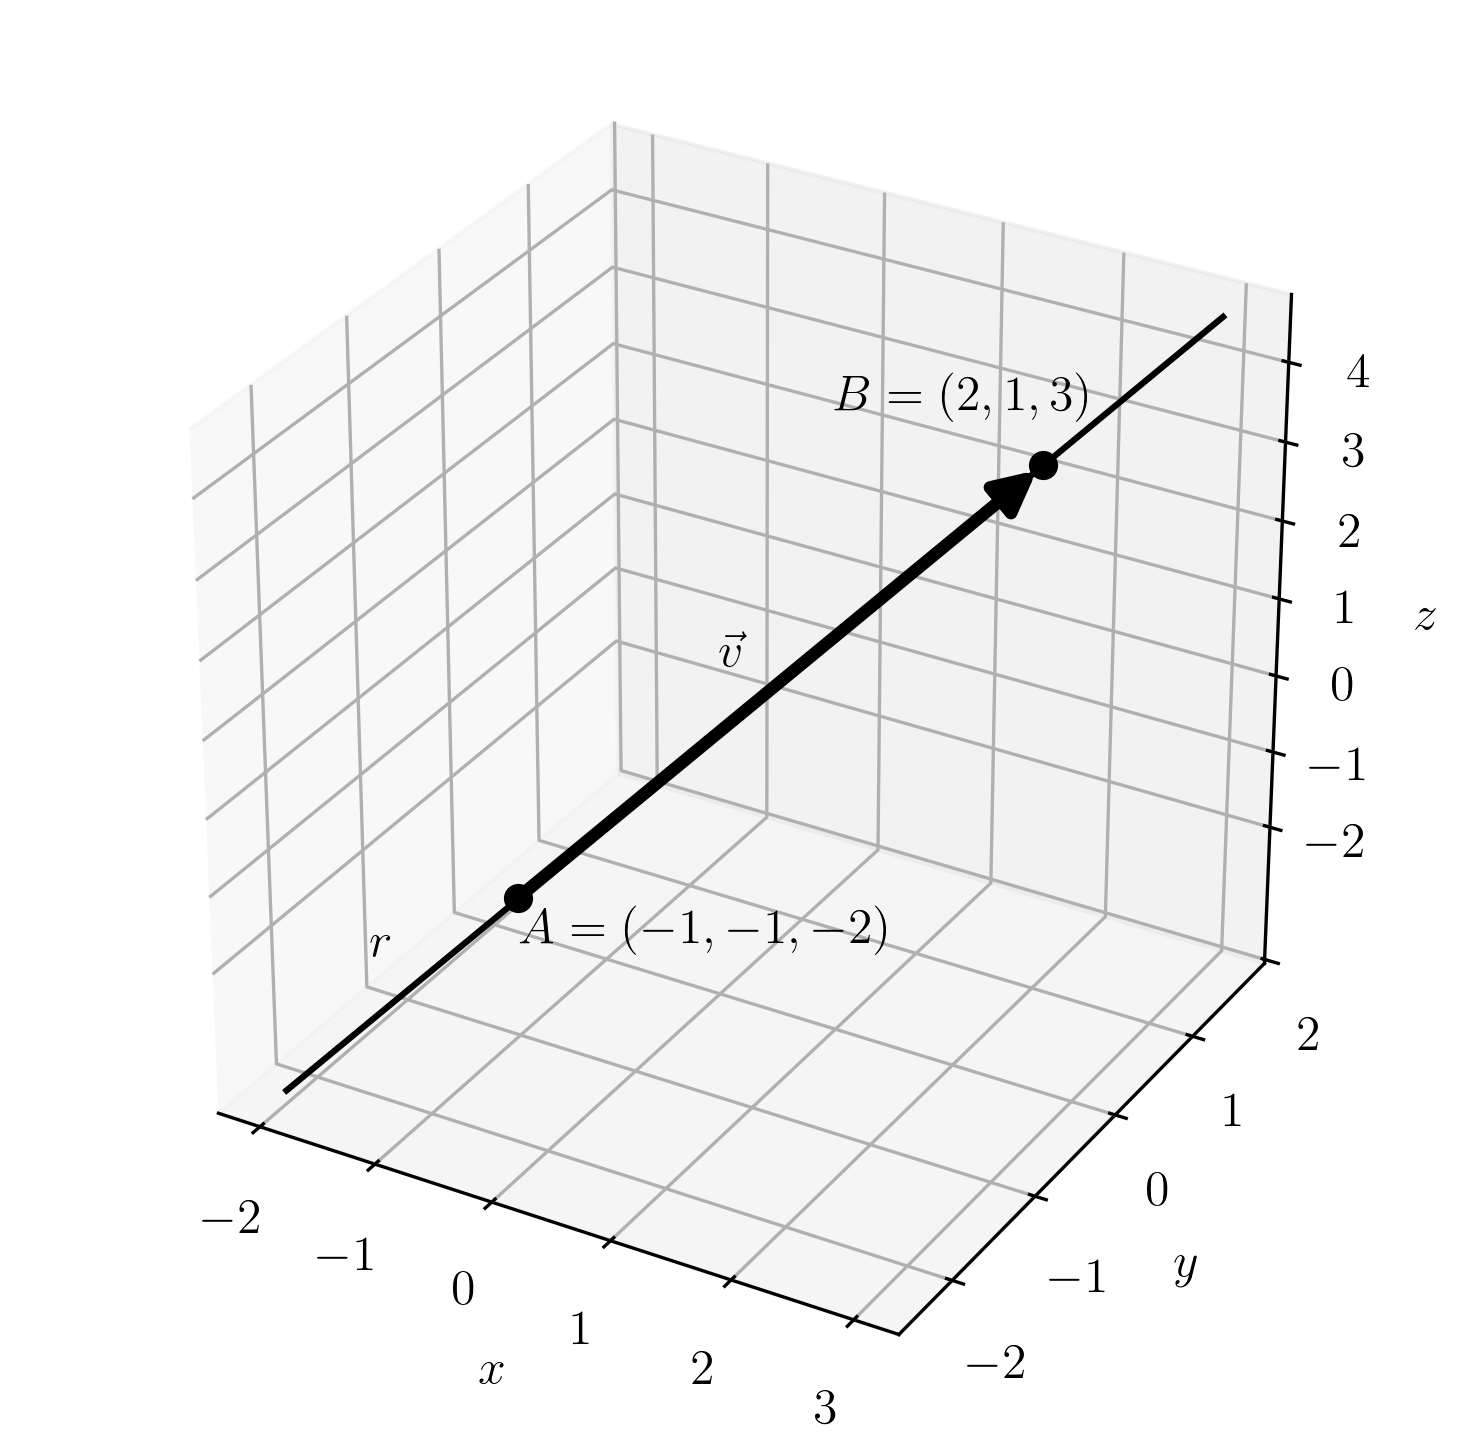
\includegraphics[width=0.7\textwidth]{./cap_er/dados/fig_ex_er_vet/fig_ex_er_vet}
    \caption{Esboço da reta discutida no Exemplo \ref{ex:er_vet}.}
    \label{fig:ex_er_vet}
  \end{figure}  
\end{ex}

\subsection{Equações paramétricas de uma reta}

Seja $r$ uma reta que passa pelo ponto $A = (x_A,y_A,z_A)$ e tenha vetor diretor $\vec{v} = (v_1,v_2,v_3)$. Assim, $P = (x,y,z)\in r$ se, e somente se, existe $\lambda\in\mathbb{R}$ tal que
\begin{equation}
  \overrightarrow{AP} = \lambda\vec{v}.
\end{equation}
Equivalentemente,
\begin{equation}
  (x-x_A,y-y_A,z-z_A) = \lambda (v_1,v_2,v_3).
\end{equation}
Então,
\begin{align}
  x-x_A &= \lambda v_1,\\
  y-y_A &= \lambda v_2,\\
  z-z_A &= \lambda v_3,
\end{align}
donde
\begin{align}
  x &= x_A + \lambda v_1,\\
  y &= y_A + \lambda v_2,\\
  z &= z_A + \lambda v_3,
\end{align}
as quais são chamadas de \emph{equações paramétricas} da reta $r$.

\begin{ex}\label{ex:ex_er_par}
  A reta $r$ discutida no Exemplo \ref{ex:er_vet} tem equações paramétricas
  \begin{align}
    x &= -1 + 3\lambda,\\
    y &= -1 + 2\lambda,\\
    z &= -2 + 5\lambda.
  \end{align}
  De fato, tomando $\lambda = 0$, temos $(x,y,z) = (-1,-1,-2) = A\in r$. E, tomado $\lambda = 1$, temos $(x,y,z) = (-1+3,-1+2,-2+5) = (2,1,3) = B\in r$. Ou seja, as equações paramétricas acima representam a reta que passa pelos pontos $A$ e $B$.

  \ifispython
  Com o \verb+Sympy+, podemos plotar o gráfico de $r$ usando o seguinte código\footnote{Veja a Observação \ref{obs:cap_er_py}.}:
\begin{verbatim}
var('lbda',real=True)
plot3d_parametric_line(-1+3*lbda,-1+2*lbda,-2+5*lbda,(lbda,-1,2))
\end{verbatim}
  \fi
\end{ex}

\subsection{Equações da reta na forma simétrica}

Seja $r$ uma reta que passa pelo ponto $A = (x_A,y_A,z_A)$ e tem $\vec{v} = (v_1,v_2,v_3)$ como vetor diretor. Então, $r$ tem as equações paramétricas
\begin{align}
  x &= x_A + v_1\lambda,\\
  y &= y_A + v_2\lambda,\\
  z &= z_A + v_3\lambda.
\end{align}
Isolando $\lambda$ em cada uma das equações, obtemos
\begin{equation}
  \frac{x-x_A}{v_1} = \frac{y-y_A}{v_2} = \frac{z-z_A}{v_3},
\end{equation}
as quais são as \emph{equações da reta na forma simétrica}.

\begin{ex}
  No Exemplo \ref{ex:ex_er_par}, consideramos a reta $r$ de equações paramétricas
  \begin{align}
    x &= -1 + 3\lambda,\\
    y &= -1 + 2\lambda,\\
    z &= -2 + 5\lambda.    
  \end{align}
  Para obtermos as equações de $r$ na forma simétrica, basta isolarmos $\lambda$ em cada equação. Com isso, obtemos
  \begin{equation}
    \frac{x+1}{3} = \frac{y+1}{2} = \frac{z+2}{5}.
  \end{equation}
\end{ex}

\subsection{Exercícios resolvidos}

\begin{exeresol}
  Seja $r$ a reta que passa pelo ponto $A = (-1,-1,-2)$ e tem $\vec{v} = (3,2,5)$ como vetor diretor. Determine o valor de $x$ de forma que $P = (x,0,1/2)$ seja um ponto de $r$.
\end{exeresol}
\begin{resol}
  $P = (x,0,1/2)$ é um ponto de $r$ se, e somente se, existe $\lambda\in\mathbb{R}$ tal que
  \begin{equation}
    \overrightarrow{AP} = \lambda\vec{v}.
  \end{equation}
  Ou seja,
  \begin{equation}
    \left(x-(-1),0-(-1),\frac{1}{2}-(-2)\right) = \lambda (3,2,5).
  \end{equation}
  Ou, equivalentemente,
  \begin{equation}
    \left(x+1,1,\frac{5}{2}\right) = \lambda (3,2,5).
  \end{equation}
  Usando a segunda coordenada destes vetores, temos
  \begin{equation}
    1 = \lambda\cdot 2 \Rightarrow \lambda = \frac{1}{2}.
  \end{equation}
  Assim, da primeira coordenada dos vetores, temos
  \begin{align}
    x+1 = \lambda 3 &\Rightarrow x+1 = \frac{3}{2}\\
                    &\Rightarrow x = \frac{3}{2}-1 = \frac{1}{2}.
  \end{align}
\end{resol}

\begin{exeresol}
  Seja $r$ a reta de equações paramétricas
  \begin{align}
    x &= 1 -\lambda,\\
    y &= \lambda,\\
    z &= -3.
  \end{align}
  Determine uma equação vetorial de $r$.
\end{exeresol}
\begin{resol}
  Nas equações paramétricas de uma reta, temos que os coeficientes constantes estão associados a um ponto da reta. Os coeficientes de $\lambda$ estão associados a um vetor diretor. Assim sendo, das equações paramétricas da reta $r$, temos que $A = (1,0,-3)\in r$ e $\vec{v} = (-1,1,0)$ é um vetor diretor. Logo, temos que a reta $r$ tem equação vetorial
  \begin{equation}
    \overrightarrow{AP} = \lambda\vec{v},
  \end{equation}
  com $A = (1,0,3)$ e $\vec{v} = (-1,1,0)$.
\end{resol}

\begin{exeresol}
  Sabendo que $r$ é uma reta que passa pelos pontos $A = (2,-3,1)$ e $B = (-1,1,0)$, determine o valor de $t$ tal que
  \begin{align}
    x = 2 + t\lambda,\\
    y = -2 + 4\lambda,\\
    z = 1 -\lambda,
  \end{align}
  sejam equação paramétricas de $r$.
\end{exeresol}
\begin{resol}
  Para que estas sejam equações paramétricas de $r$, é necessário que $\vec{v} = (t,4,-1)$ seja um vetor diretor de $r$. Em particular, $\vec{v} \parallel \overrightarrow{AB}$. Logo, existe $\beta\in\mathbb{R}$ tal que
  \begin{equation}
    (t,4,-1) = \beta (-1-2,1-(-3),0-1) = \beta (-3,4,-1).
  \end{equation}
  Das segunda e terceira coordenadas, temos $\beta = 1$. Daí, comparando pela primeira coordenada, temos
  \begin{equation}
    t = -3\beta \Rightarrow t = -3.
  \end{equation}
\end{resol}

\begin{exeresol}\label{exeresol:er_sim}
  Seja $r$ uma reta, cujas equações na forma simétrica são
  \begin{equation}
    \frac{x+1}{2} = \frac{y-2}{3} = \frac{1-z}{2}.
  \end{equation}
  Determine equações paramétricas desta reta e faça um esboço de seu gráfico.
\end{exeresol}
\begin{resol}
  Podemos obter equações paramétricas desta reta a partir de suas equações na forma simétrica. Para tanto, basta tomar o parâmetro $\lambda$ tal que
  \begin{align}
    \lambda &= \frac{x+1}{2},\\
    \lambda &= \frac{y-2}{3},\\
    \lambda &= \frac{1-z}{2}.
  \end{align}
  Daí, isolando $x$, $y$ e $z$ em cada uma destas equações, obtemos
  \begin{align}
    x &= -1 + 2\lambda,\\
    y &= 2 + 3\lambda,\\
    z &= 1 - 2\lambda.
  \end{align}
  Para fazermos um esboço do gráfico desta reta, basta traçarmos a reta que passa por dois de seus pontos. Por exemplo, tomando $\lambda = 0$, temos $A = (-1,2,1)\in r$. Agora, tomando $\lambda = 1$, temos $B = (1,5,-1)\in r$. Desta forma, obtemos o esboço dado na Figura \ref{fig:exeresol_er_sim}.

  \begin{figure}[H]
    \centering
    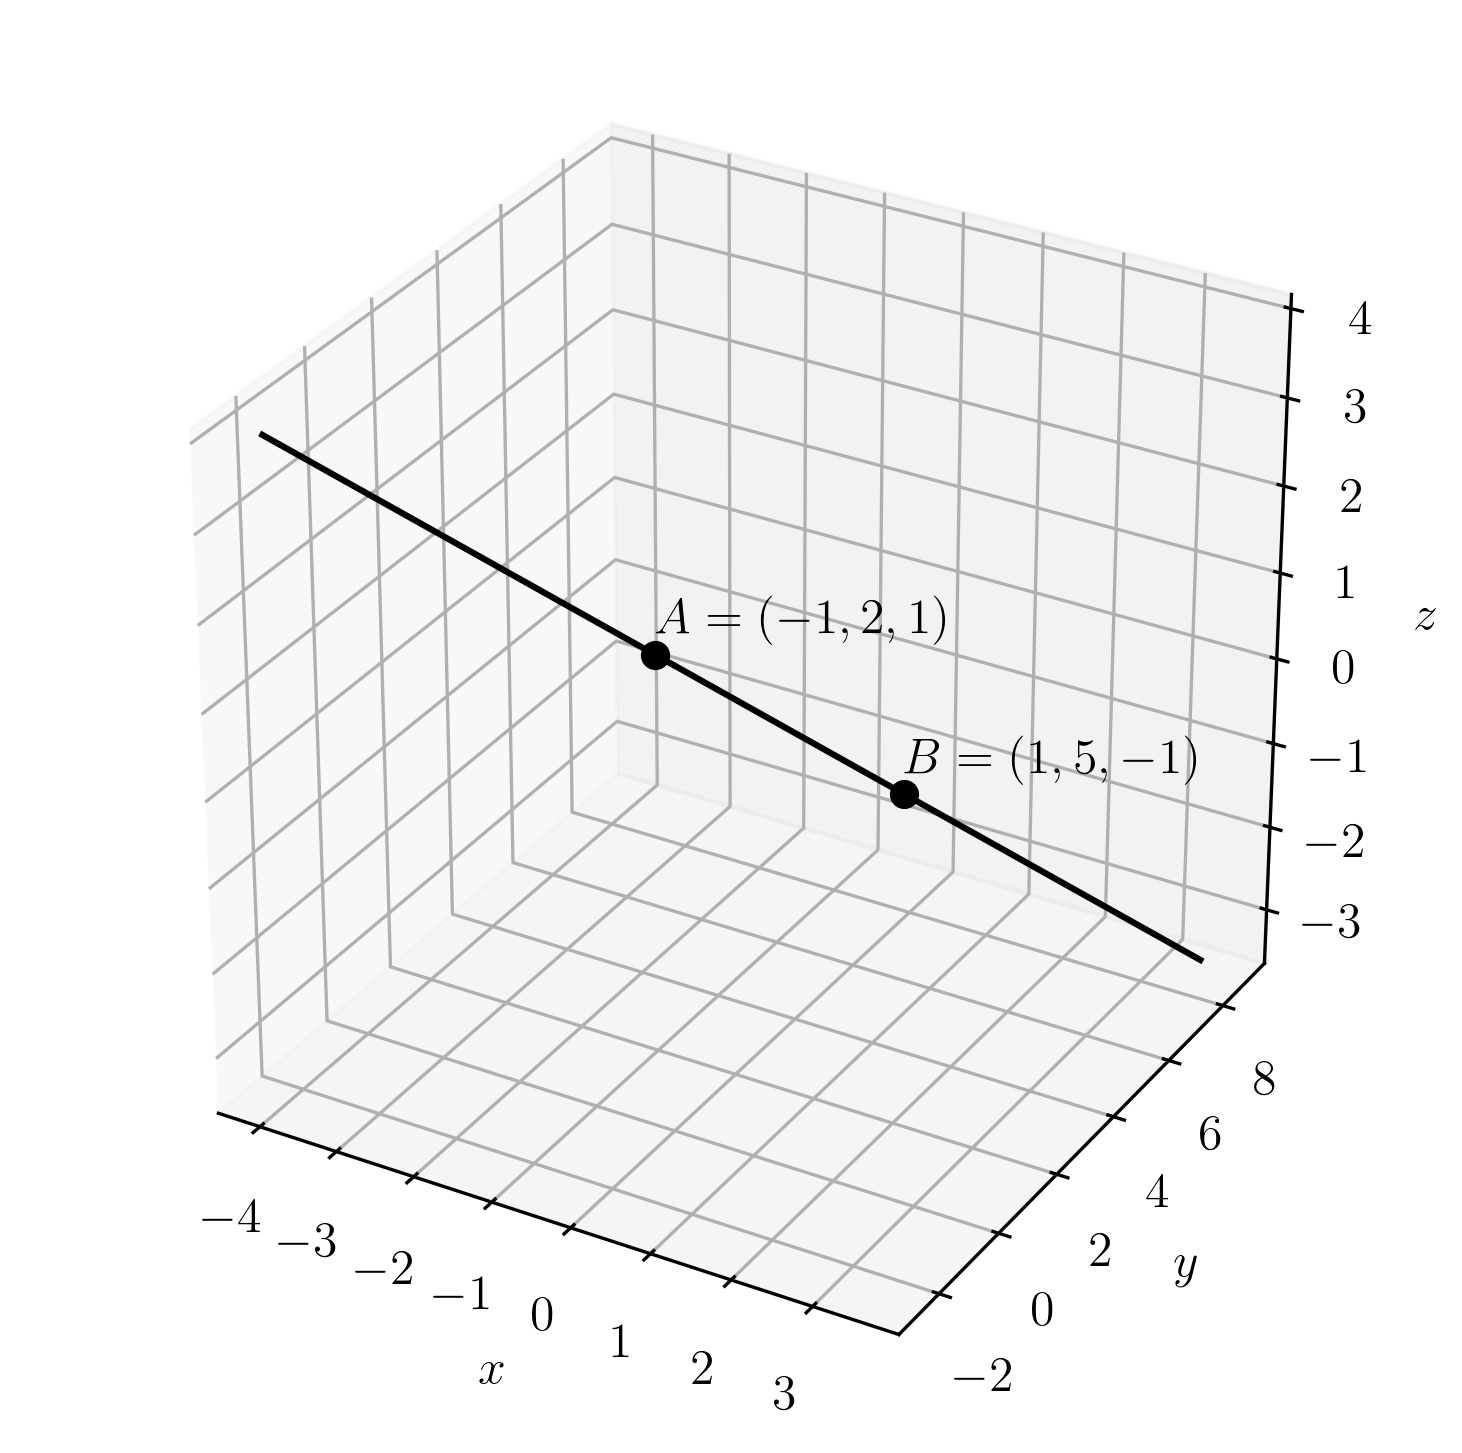
\includegraphics[width=0.7\textwidth]{./cap_er/dados/fig_exeresol_er_sim/fig_exeresol_er_sim}
    \caption{Esboço do gráfico da reta $r$ do Exercício Resolvido \ref{exeresol:er_sim}.}
    \label{fig:exeresol_er_sim}
  \end{figure}
\end{resol}
%Este trabalho está licenciado sob a Licença Atribuição-CompartilhaIgual 4.0 Internacional Creative Commons. Para visualizar uma cópia desta licença, visite http://creativecommons.org/licenses/by-sa/4.0/deed.pt_BR ou mande uma carta para Creative Commons, PO Box 1866, Mountain View, CA 94042, USA.

\chapter{Estudo de retas}\label{cap_er}
\thispagestyle{fancy}

\ifispython
\begin{obs}\label{obs:cap_er_py}
  Neste capítulo, assumimos que os códigos \verb+Python+ têm o seguinte preambulo:
\begin{verbatim}
from sympy import *
from sympy.plotting import plot3d_parametric_line
\end{verbatim}
\end{obs}
\fi

\section{Sistema de coordenadas no espaço}\label{cap_er_sec_siscoord}

Um sistema de coordenadas no espaço é constituído de um ponto $O$ e uma base de vetores $B = (\vec{e}_1, \vec{e}_2, \vec{e}_3)$ no espaço. Dado um tal sistema, temos que cada ponto $P$ determina de forma única um vetor $\overrightarrow{OP} = (x,y,z)$ e vice-versa. Assim sendo, definimos que o ponto $P$ tem coordenadas $(x,y,z)$.

O ponto $O$ é chamado de \emph{origem} (do sistema de coordenados) e tem coordenadas $(0,0,0)$. Dado um ponto $P=(x,y,z)$, chama-se $x$ de sua \emph{abscissa}, $y$ de sua \emph{ordenada} e $z$ de sua \emph{cota}. As retas que passam por $O$ e têm, respectivamente, as mesmas direções de $\vec{e}_1$, $\vec{e}_2$ e $\vec{e}_3$ são chamadas de \emph{eixo das abscissas}, \emph{eixo das ordenadas} e \emph{eixo das cotas}. Os planos que contém $O$ e representantes de dois vetores da base $B$ são chamados de \emph{planos coordenados}.

\begin{figure}[H]
  \centering
  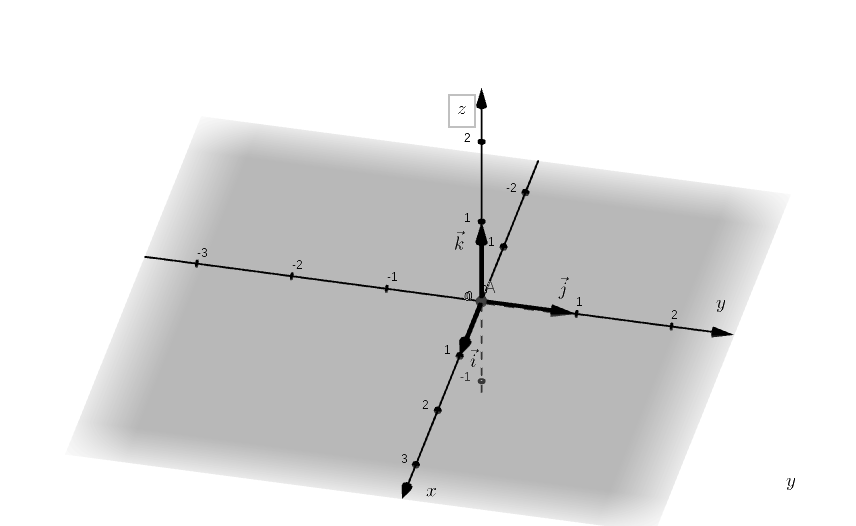
\includegraphics[width=0.7\textwidth]{./cap_er/dados/fig_sis_coord_orto/fig_sis_coord_orto}
  \caption{Sistema de coordenadas ortonormal.}
  \label{fig:sis_coord_orto}
\end{figure}

Salvo explicitado ao contrário, trabalharemos com \emph{sistemas de coordenadas ortogonais}, i.e. sistema cuja base $B = (\vec{i},\vec{j},\vec{k})$ seja ortonormal. Mais ainda, estaremos assumindo que a base é positiva. Veja a Figura \ref{fig:sis_coord_orto}.

\begin{obs}\normalfont{(Relação entre pontos e vetores)}
  Seja dado um vetor $\overrightarrow{AB}$. Sabendo as coordenadas dos pontos $A = (x_A,y_A,z_A)$ e $B = (x_B,y_B,z_B)$, temos que as coordenadas do vetor $\overrightarrow{AB}$ são:
  \begin{align}
    \overrightarrow{AB} &= \overrightarrow{AO} + \overrightarrow{OB}\\
                        &= -\overrightarrow{OA} + \overrightarrow{OB}\\
                        &= -(x_A,y_A,z_A)+(x_B,y_B,z_B)\\
                        &= (x_B-x_A,y_B-y_A,z_B-z_A).
  \end{align}
\end{obs}

\begin{ex}
  Dados os pontos $A = (-1,1,2)$ e $B = (3,-1,0)$, temos que o vetor $\overrightarrow{AB}$ tem coordenadas:
  \begin{equation}
    \overrightarrow{AB} = (3-(-1),-1-1,0-2) = (4,-2,-2).
  \end{equation}
\end{ex}

\begin{obs}\normalfont{(Ponto médio de um segmento)}
  Dados os pontos $A = (x_A,y_A,z_A)$ e $B = (x_B,y_B,z_B)$, podemos calcular as coordenadas do ponto médio $M = (x_M,y_M,z_M)$ do segmento $AB$, do fato de que $\overrightarrow{AM} = \overrightarrow{MB}$. Portanto
  \begin{equation}
    (x_M-x_A,y_M-y_A,z_M-z_A)=(x_B-x_M,y_B-y_M,z_B-z_M),
  \end{equation}
  donde
  \begin{align}
    2x_M &= x_A+x_B\\
    2y_M &= y_A+y_B\\
    2z_M &= z_A+z_B.
  \end{align}
  Logo, temos $\displaystyle M = \left(\frac{x_A+x_B}{2},\frac{y_A+y_B}{2},\frac{z_A+z_B}{2}\right)$.
\end{obs}

\begin{ex}
  Dados os pontos $A = (-1,1,2)$ e $B = (3,-1,0)$, temos que o ponto médio do segmento $AB$ tem coordenadas:
  \begin{equation}
    M = \left(\frac{-1+3}{2},\frac{1+(-1)}{2},\frac{2+0}{2}\right) = (1,0,1).
  \end{equation}
\end{ex}

\subsection*{Exercícios resolvidos}

\begin{exeresol}
  Sejam $A = (-1,2,1)$, $B = (1,-2,0)$ e $C = (x,2,2)$ vértices consecutivos de um triângulo isósceles, cujos lados $AC$ e $BC$ são congruentes. Determine o valor de $x$.
\end{exeresol}
\begin{resol}
  Sendo os lados $AC$ e $BC$ congruentes, temos $|\overrightarrow{AC}| = |\overrightarrow{BC}|$. As coordenadas de $\overrightarrow{AC}$ são
  \begin{equation}
    \overrightarrow{AC} = (x-(-1),2-2,2-1) = (x+1,0,1)
  \end{equation}
  e as coordenadas de $\overrightarrow{BC}$ são
  \begin{equation}
    \overrightarrow{BC} = (x-1,2-(-2),2-0) = (x-1,4,2).
  \end{equation}
  Então, temos
  \begin{align}
    |\overrightarrow{AC}| = |\overrightarrow{BC}| &\Rightarrow \sqrt{(x+1)^2+0^2+1^2} = \sqrt{(x-1)^2+4^2+2^2}\\
                                                  &\Rightarrow (x+1)^2+0^2+1^2 = (x-1)^2+4^2+2^2\\
                                                  &\Rightarrow x^2+2x+1+1 = x^2-2x+1+16+4\\
                                                  &\Rightarrow 4x = 19\\
                                                  &\Rightarrow x = \frac{19}{4}.
  \end{align}
\end{resol}

\begin{exeresol}
  Sejam $A = (-1,2,1)$, $B = (1,-2,0)$  e $M$ o ponto médio do intervalo $AB$. Determine as coordenadas do ponto $P$ de forma que $2AP = AM$.
\end{exeresol}
\begin{resol}
  As coordenadas do ponto médio são
  \begin{equation}
    M = \left(\frac{-1+1}{2},\frac{2+(-2)}{2},\frac{1+0}{2}\right) = \left(0,0,\frac{1}{2}\right).
  \end{equation}
  Agora, denotando $P = (x_P,y_P,z_P)$, temos
  \begin{align}
    2AP = AM &\Rightarrow 2(x_P-(-1),y_P-2,z_P-1) = \left(0-(-1),0-2,\frac{1}{2}-1\right)\\
             &\Rightarrow (2x_p+2,2y_P-4,2z_P-2) = \left(1,-2,-\frac{1}{2}\right).
  \end{align}
  Portanto
  \begin{align}
    & 2x_P+2 = 1 \Rightarrow x_P = -\frac{1}{2}\\
    & 2y_P-4 = -2 \Rightarrow y_P = 1\\
    & 2z_P-2 = -\frac{1}{2} \Rightarrow z_P = \frac{3}{4}.
  \end{align}
  Logo, $P = (-1/2,1,3/4)$.
\end{resol}

\subsection*{Exercícios}

\emconstrucao

\section{Equações da reta}\label{cap_ert_sec_eqsreta}

\subsection{Equação vetorial de uma reta}

Seja $r$ uma reta dada, $\vec{v}$ um vetor paralelo a $r$ e $A$ um ponto de $r$ (veja a Figura~\ref{fig:er_vet}). Assim sendo, $P$ é um ponto de $r$ se, e somente se, existe $\lambda\in\mathbb{R}$ tal que
\begin{equation}
  \overrightarrow{AP} = \lambda\vec{v}.
\end{equation}
Esta é chamada \emph{equação vetorial da reta} $r$.

\begin{figure}[H]
  \centering
  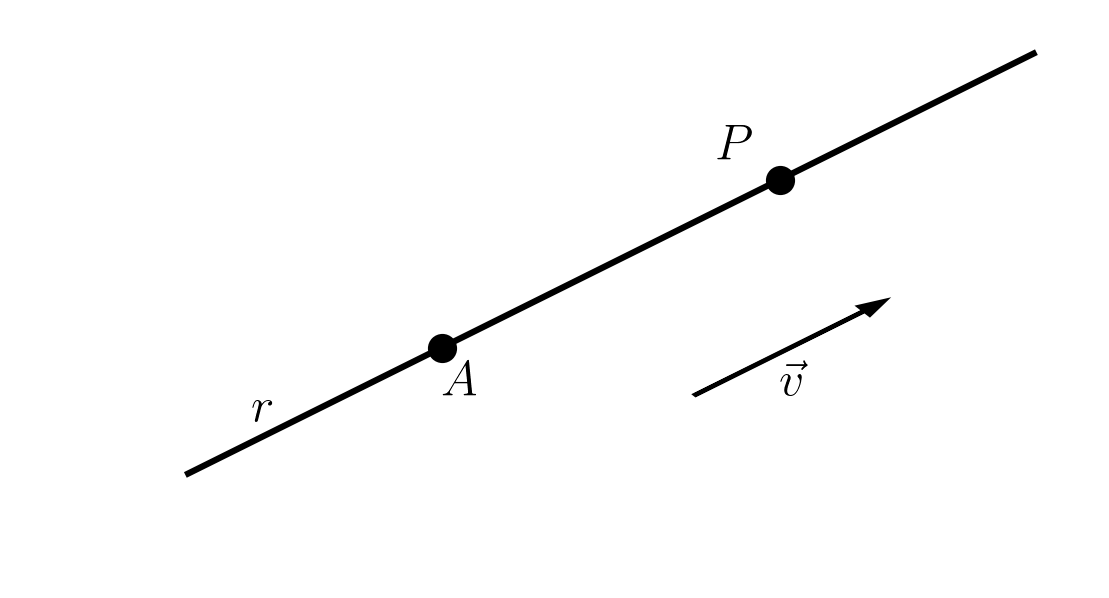
\includegraphics[width=0.5\textwidth]{./cap_er/dados/fig_er_vet/fig_er_vet}
  \caption{Equação vetorial de uma reta.}
  \label{fig:er_vet}
\end{figure}

Observe que para obtermos uma equação vetorial de uma dada reta, podemos escolher qualquer ponto $A\in r$ e qualquer vetor $\vec{v}\parallel r$, $\vec{v}\neq\vec{0}$. O vetor $\vec{v}$ escolhido é chamado de \emph{vetor diretor}.

\begin{ex}\label{ex:er_vet}
  Seja $r$ a reta que passa pelos pontos $A=(-1,-1,-2)$ e $B = (2,1,3)$ (veja a Figura \ref{fig:ex_er_vet}). O vetor
  \begin{equation}
    \vec{v} = \overrightarrow{AB} = (2-(-1),1-(-1),3-(-2)) = (3,2,5)
  \end{equation}
  é um vetor diretor de $r$. Desta forma, uma equação vetorial da reta $r$ é
  \begin{equation}
    \overrightarrow{AP} = \lambda\vec{v}.
  \end{equation}
  \begin{figure}[H]
    \centering
    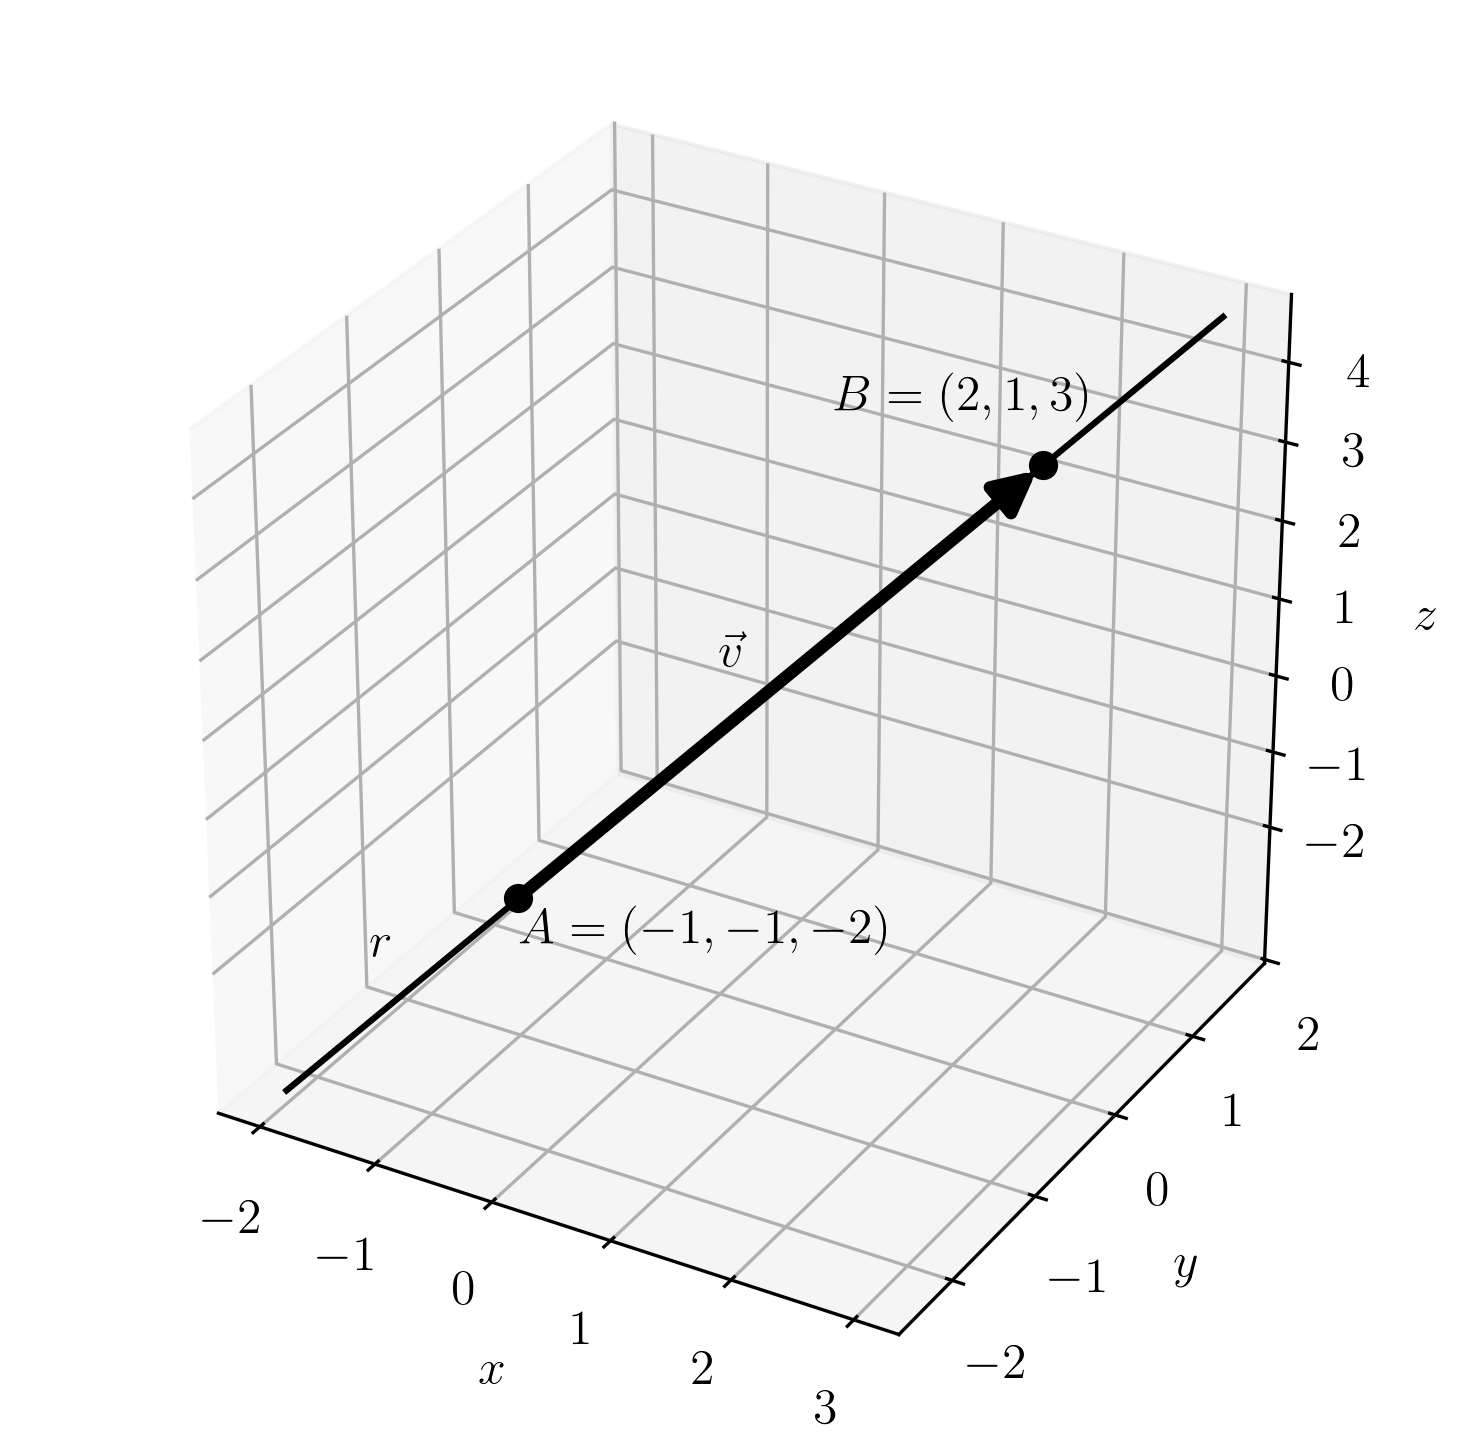
\includegraphics[width=0.7\textwidth]{./cap_er/dados/fig_ex_er_vet/fig_ex_er_vet}
    \caption{Esboço da reta discutida no Exemplo \ref{ex:er_vet}.}
    \label{fig:ex_er_vet}
  \end{figure}  
\end{ex}

\subsection{Equações paramétricas de uma reta}

Seja $r$ uma reta que passa pelo ponto $A = (x_A,y_A,z_A)$ e tenha vetor diretor $\vec{v} = (v_1,v_2,v_3)$. Assim, $P = (x,y,z)\in r$ se, e somente se, existe $\lambda\in\mathbb{R}$ tal que
\begin{equation}
  \overrightarrow{AP} = \lambda\vec{v}.
\end{equation}
Equivalentemente,
\begin{equation}
  (x-x_A,y-y_A,z-z_A) = \lambda (v_1,v_2,v_3).
\end{equation}
Então,
\begin{align}
  x-x_A &= \lambda v_1,\\
  y-y_A &= \lambda v_2,\\
  z-z_A &= \lambda v_3,
\end{align}
donde
\begin{align}
  x &= x_A + \lambda v_1,\\
  y &= y_A + \lambda v_2,\\
  z &= z_A + \lambda v_3,
\end{align}
as quais são chamadas de \emph{equações paramétricas} da reta $r$.

\begin{ex}\label{ex:ex_er_par}
  A reta $r$ discutida no Exemplo \ref{ex:er_vet} tem equações paramétricas
  \begin{align}
    x &= -1 + 3\lambda,\\
    y &= -1 + 2\lambda,\\
    z &= -2 + 5\lambda.
  \end{align}
  De fato, tomando $\lambda = 0$, temos $(x,y,z) = (-1,-1,-2) = A\in r$. E, tomado $\lambda = 1$, temos $(x,y,z) = (-1+3,-1+2,-2+5) = (2,1,3) = B\in r$. Ou seja, as equações paramétricas acima representam a reta que passa pelos pontos $A$ e $B$.

  \ifispython
  Com o \verb+Sympy+, podemos plotar o gráfico de $r$ usando o seguinte código\footnote{Veja a Observação \ref{obs:cap_er_py}.}:
\begin{verbatim}
var('lbda',real=True)
plot3d_parametric_line(-1+3*lbda,-1+2*lbda,-2+5*lbda,(lbda,-1,2))
\end{verbatim}
  \fi
\end{ex}

\subsection{Equações da reta na forma simétrica}

Seja $r$ uma reta que passa pelo ponto $A = (x_A,y_A,z_A)$ e tem $\vec{v} = (v_1,v_2,v_3)$ como vetor diretor. Então, $r$ tem as equações paramétricas
\begin{align}
  x &= x_A + v_1\lambda,\\
  y &= y_A + v_2\lambda,\\
  z &= z_A + v_3\lambda.
\end{align}
Isolando $\lambda$ em cada uma das equações, obtemos
\begin{equation}
  \frac{x-x_A}{v_1} = \frac{y-y_A}{v_2} = \frac{z-z_A}{v_3},
\end{equation}
as quais são as \emph{equações da reta na forma simétrica}.

\begin{ex}
  No Exemplo \ref{ex:ex_er_par}, consideramos a reta $r$ de equações paramétricas
  \begin{align}
    x &= -1 + 3\lambda,\\
    y &= -1 + 2\lambda,\\
    z &= -2 + 5\lambda.    
  \end{align}
  Para obtermos as equações de $r$ na forma simétrica, basta isolarmos $\lambda$ em cada equação. Com isso, obtemos
  \begin{equation}
    \frac{x+1}{3} = \frac{y+1}{2} = \frac{z+2}{5}.
  \end{equation}
\end{ex}

\subsection{Exercícios resolvidos}

\begin{exeresol}
  Seja $r$ a reta que passa pelo ponto $A = (-1,-1,-2)$ e tem $\vec{v} = (3,2,5)$ como vetor diretor. Determine o valor de $x$ de forma que $P = (x,0,1/2)$ seja um ponto de $r$.
\end{exeresol}
\begin{resol}
  $P = (x,0,1/2)$ é um ponto de $r$ se, e somente se, existe $\lambda\in\mathbb{R}$ tal que
  \begin{equation}
    \overrightarrow{AP} = \lambda\vec{v}.
  \end{equation}
  Ou seja,
  \begin{equation}
    \left(x-(-1),0-(-1),\frac{1}{2}-(-2)\right) = \lambda (3,2,5).
  \end{equation}
  Ou, equivalentemente,
  \begin{equation}
    \left(x+1,1,\frac{5}{2}\right) = \lambda (3,2,5).
  \end{equation}
  Usando a segunda coordenada destes vetores, temos
  \begin{equation}
    1 = \lambda\cdot 2 \Rightarrow \lambda = \frac{1}{2}.
  \end{equation}
  Assim, da primeira coordenada dos vetores, temos
  \begin{align}
    x+1 = \lambda 3 &\Rightarrow x+1 = \frac{3}{2}\\
                    &\Rightarrow x = \frac{3}{2}-1 = \frac{1}{2}.
  \end{align}
\end{resol}

\begin{exeresol}
  Seja $r$ a reta de equações paramétricas
  \begin{align}
    x &= 1 -\lambda,\\
    y &= \lambda,\\
    z &= -3.
  \end{align}
  Determine uma equação vetorial de $r$.
\end{exeresol}
\begin{resol}
  Nas equações paramétricas de uma reta, temos que os coeficientes constantes estão associados a um ponto da reta. Os coeficientes de $\lambda$ estão associados a um vetor diretor. Assim sendo, das equações paramétricas da reta $r$, temos que $A = (1,0,-3)\in r$ e $\vec{v} = (-1,1,0)$ é um vetor diretor. Logo, temos que a reta $r$ tem equação vetorial
  \begin{equation}
    \overrightarrow{AP} = \lambda\vec{v},
  \end{equation}
  com $A = (1,0,3)$ e $\vec{v} = (-1,1,0)$.
\end{resol}

\begin{exeresol}
  Sabendo que $r$ é uma reta que passa pelos pontos $A = (2,-3,1)$ e $B = (-1,1,0)$, determine o valor de $t$ tal que
  \begin{align}
    x = 2 + t\lambda,\\
    y = -2 + 4\lambda,\\
    z = 1 -\lambda,
  \end{align}
  sejam equação paramétricas de $r$.
\end{exeresol}
\begin{resol}
  Para que estas sejam equações paramétricas de $r$, é necessário que $\vec{v} = (t,4,-1)$ seja um vetor diretor de $r$. Em particular, $\vec{v} \parallel \overrightarrow{AB}$. Logo, existe $\beta\in\mathbb{R}$ tal que
  \begin{equation}
    (t,4,-1) = \beta (-1-2,1-(-3),0-1) = \beta (-3,4,-1).
  \end{equation}
  Das segunda e terceira coordenadas, temos $\beta = 1$. Daí, comparando pela primeira coordenada, temos
  \begin{equation}
    t = -3\beta \Rightarrow t = -3.
  \end{equation}
\end{resol}

\begin{exeresol}\label{exeresol:er_sim}
  Seja $r$ uma reta, cujas equações na forma simétrica são
  \begin{equation}
    \frac{x+1}{2} = \frac{y-2}{3} = \frac{1-z}{2}.
  \end{equation}
  Determine equações paramétricas desta reta e faça um esboço de seu gráfico.
\end{exeresol}
\begin{resol}
  Podemos obter equações paramétricas desta reta a partir de suas equações na forma simétrica. Para tanto, basta tomar o parâmetro $\lambda$ tal que
  \begin{align}
    \lambda &= \frac{x+1}{2},\\
    \lambda &= \frac{y-2}{3},\\
    \lambda &= \frac{1-z}{2}.
  \end{align}
  Daí, isolando $x$, $y$ e $z$ em cada uma destas equações, obtemos
  \begin{align}
    x &= -1 + 2\lambda,\\
    y &= 2 + 3\lambda,\\
    z &= 1 - 2\lambda.
  \end{align}
  Para fazermos um esboço do gráfico desta reta, basta traçarmos a reta que passa por dois de seus pontos. Por exemplo, tomando $\lambda = 0$, temos $A = (-1,2,1)\in r$. Agora, tomando $\lambda = 1$, temos $B = (1,5,-1)\in r$. Desta forma, obtemos o esboço dado na Figura \ref{fig:exeresol_er_sim}.

  \begin{figure}[H]
    \centering
    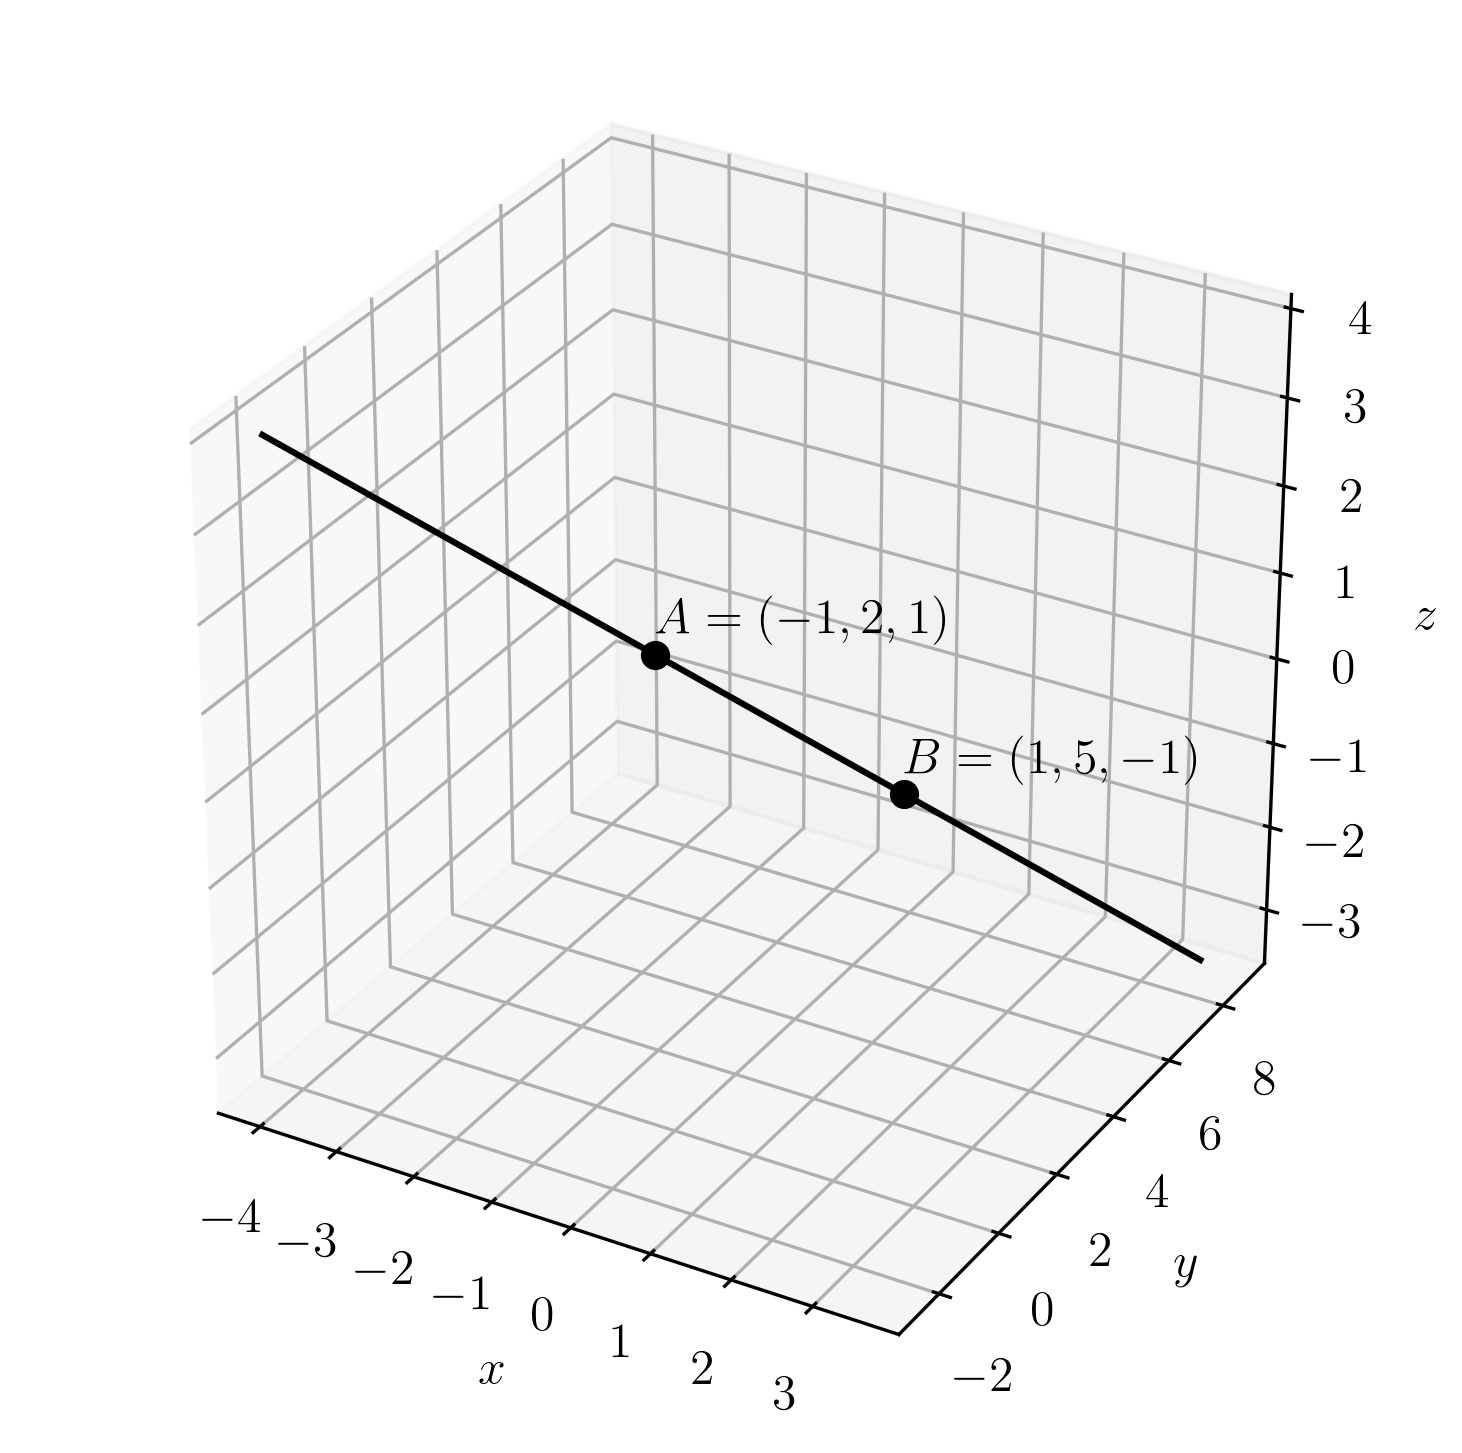
\includegraphics[width=0.7\textwidth]{./cap_er/dados/fig_exeresol_er_sim/fig_exeresol_er_sim}
    \caption{Esboço do gráfico da reta $r$ do Exercício Resolvido \ref{exeresol:er_sim}.}
    \label{fig:exeresol_er_sim}
  \end{figure}
\end{resol}
%Este trabalho está licenciado sob a Licença Atribuição-CompartilhaIgual 4.0 Internacional Creative Commons. Para visualizar uma cópia desta licença, visite http://creativecommons.org/licenses/by-sa/4.0/deed.pt_BR ou mande uma carta para Creative Commons, PO Box 1866, Mountain View, CA 94042, USA.

\chapter{Estudo de planos}\label{cap_ep}
\thispagestyle{fancy}

Neste capítulo, temos uma introdução ao estudo de planos no espaço tridimensional.

\section{Equações do plano}\label{cap_ep_sec_eqsplano}

Um plano $\pi$ fica unicamente determinado por um ponto $A\in \pi$ e dois vetores linearmente independentes $\vec{u},\vec{v}\in \pi$\footnote{No sentido que $\vec{u}$ e $\vec{v}$ têm representantes no plano $\pi$.}. Veja a Figura \ref{fig:ep_plano}.

\begin{figure}[H]
  \centering
  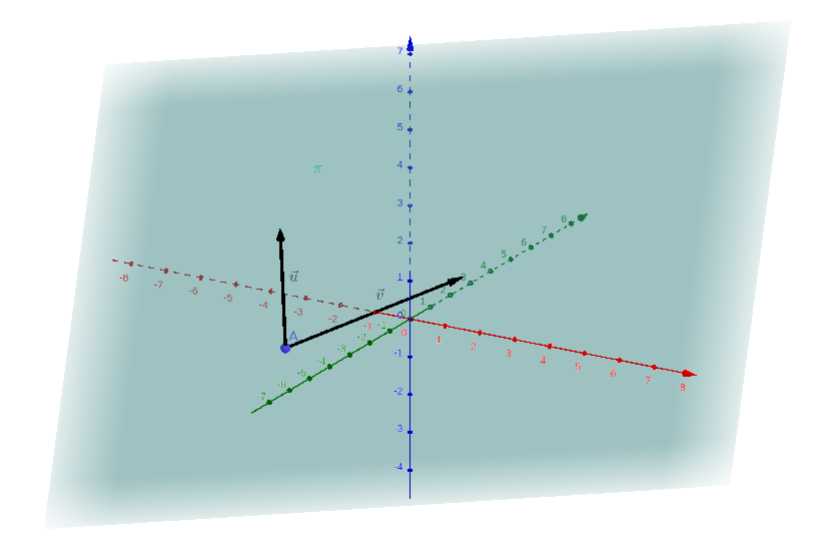
\includegraphics[width=0.9\textwidth]{cap_ep/dados/fig_ep_plano/fig}
  \caption{Ilustração de um plano no espaço tridimensional.}
  \label{fig:ep_plano}
\end{figure}

Os chamados \emph{vetores diretores} $\vec{u}$ e $\vec{v}$ determinam infinitos planos paralelos entre si. O chamado \emph{ponto de ancoragem} $A$ fixa um destes planos.

\subsection{Equação vetorial do plano}

Consideremos um plano $\pi$ determinado pelo ponto de ancoragem $A$ e os vetores diretores $\vec{u}$ e $\vec{v}$ (veja a Figura \ref{fig:ep_evp}). Então, um ponto $P\in \pi$ se, e somente se, $\overrightarrow{AP}$ é coplanar a $\vec{u}$ e $\vec{v}$, i.e. $\overrightarrow{AP}$, $\vec{u}$ e $\vec{v}$ são linearmente dependentes. Ou seja, $P\in\pi$ se, e somente se, $\overrightarrow{AP}$ pode ser escrito como combinação linear de $\vec{u}$ e $\vec{v}$. Isto nos fornece a chamada \emph{equação vetorial do plano}
\begin{equation}
  {\color{blue}P\in\pi \Leftrightarrow \overrightarrow{AP} = \lambda\vec{u}+\beta\vec{v},\quad\lambda,\beta\in\mathbb{R}}.
\end{equation}

\begin{figure}[H]
  \centering
  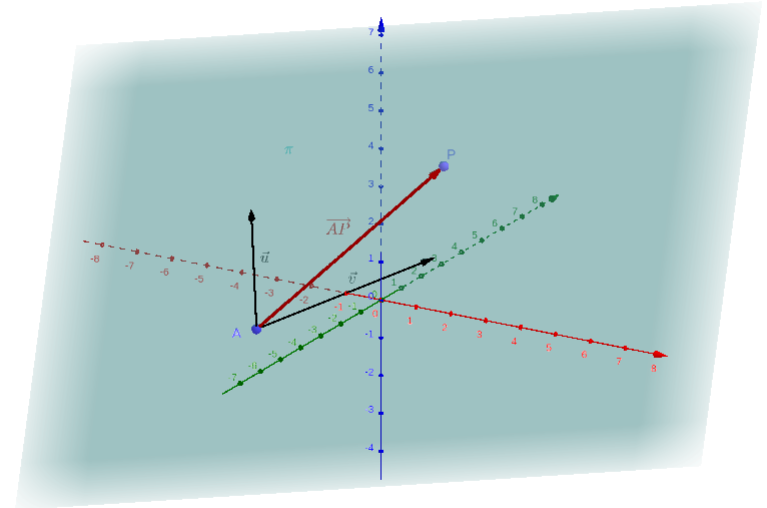
\includegraphics[width=0.9\textwidth]{cap_ep/dados/fig_ep_evp/fig}
  \caption{Ilustração sobre a equação vetorial de um plano.}
  \label{fig:ep_evp}
\end{figure}


\begin{ex}\label{ex:ep_vet}
  Consideremos o plano $\pi$ determinado pelo ponto $A = (1,-1,1)$ e pelos vetores $\vec{u} = (2,-1,0)$ e $\vec{v} = (0,1,1)$ (Veja a Figura \ref{fig:ex_ep_vet}. Desta forma, uma equação vetorial para este plano é
  \begin{equation}
    \overrightarrow{AP} = \lambda\vec{u}+\beta\vec{v},
  \end{equation}
  para $\lambda,\beta\in\mathbb{R}$.
  
  \begin{figure}[H]
    \centering
    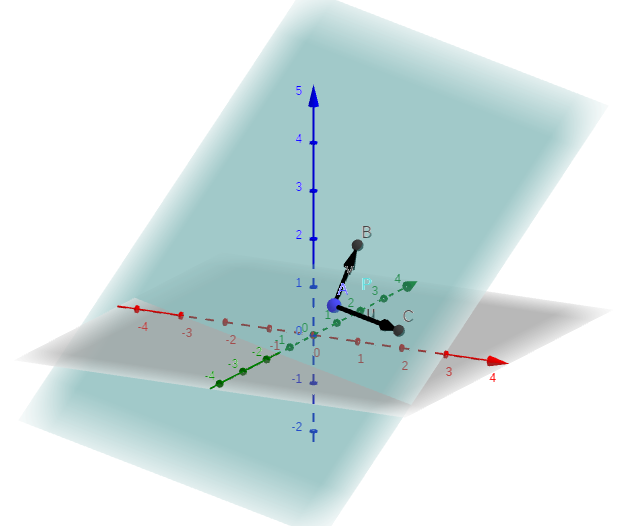
\includegraphics[width=0.9\textwidth]{./cap_ep/dados/fig_ex_ep_vet/fig_ex_ep_vet}
    \caption{Esboço do plano $\pi$ discutido no Exemplo \ref{ex:ep_vet}.}
    \label{fig:ex_ep_vet}
  \end{figure}
  
  Tomando, por exemplo, $\lambda = -1$ e $\beta = 1$, obtemos
  \begin{align}
    \overrightarrow{AP} &= \lambda\vec{u}+\beta\vec{v}\\
                        &= -(2,-1,0) + (0,1,1)\\
                        &= (-2,2,1).
  \end{align}
  Observando que as coordenadas do ponto $P$ são iguais as coordenadas do vetor $\overrightarrow{OP}$, temos
  \begin{align}
    \overrightarrow{OP} &= \overrightarrow{OA}+\overrightarrow{AP}\\
                        &= (1,-1,1)+(-2,2,1)\\
                        &= (-1,1,2).
  \end{align}
  Ou seja, $P = (-1,1,2)\in\pi$.
\end{ex}

\subsection{Equações paramétricas do plano}

Seja um plano $\pi$ com ponto de ancoragem $A=(x_A,y_A,z_A)\in\pi$ e vetores diretores $\vec{u}=(u_1,u_2,u_3)$ e $\vec{v}=(v_1,v_2,v_3)$. Então, todo o ponto $P=(x,y,z)$ neste plano $\pi$ satisfaz a equação vetorial
\begin{equation}
  \overrightarrow{AP} = \lambda\vec{u}+\beta\vec{v},
\end{equation}
para dados parâmetros $\lambda,\beta\in\mathbb{R}$. Assim, temos
\begin{align}
  (x-x_A,y-y_A,z-z_A) &= \lambda(u_1,u_2,u_3)+\beta(v_1,v_2,v_3)\\
                      &= (\lambda u_1+\beta v_1,\lambda u_2+\beta v_2,\lambda u_3+\beta v_3).
\end{align}
Portanto, temos
\begin{align}
  x-x_A &= \lambda u_1+\beta v_1,\\
  y-y_A &= \lambda u_2+\beta v_2,\\
  z-z_A &= \lambda u_3+\beta v_3.
\end{align}
Ou, equivalentemente,
\begin{align}
  {\color{blue}x} &= {\color{blue}x_A + \lambda u_1+\beta v_1},\\
  {\color{blue}y} &= {\color{blue}y_A + \lambda u_2+\beta v_2},\\
  {\color{blue}z} &= {\color{blue}z_A + \lambda u_3+\beta v_3},
\end{align}
as quais são chamadas de \emph{equações paramétricas do plano}.

\begin{ex}
  No Exemplo \ref{ex:ep_vet}, discutimos sobre o plano $\pi$ determinado pelo ponto $A = (1,-1,1)$ e os vetores $\vec{u}=(2,-1,0)$ e $\vec{v}=(0,1,1)$. Do que vimos acima, temos que
  \begin{align}
    x &= 1 + 2\lambda,\\
    y &= -1 -\lambda + \beta,\\
    z &= 1+\beta,
  \end{align}
  são equações paramétricas deste plano.

  \ifispython
  Podemos usar as equações paramétricas do plano para plotá-lo usando o \sympy. Para tanto, podemos usar os seguintes comandos:
\begin{verbatim}
from sympy import *
from sympy.plotting import plot3d_parametric_surface
var('r,s',real=True)
plot3d_parametric_surface(1+2*r,-1-r+s,1+s,
                          (r,-2,2),(s,-2,2),show=True,
                          xlabel='$x$',ylabel='$y$')
\end{verbatim}
  \fi
\end{ex}

\subsection{Equação geral do plano}

Seja $\pi$ o plano determinado pelo ponto de ancoragem $A=(x_A,y_A,z_A)$ e pelos vetores diretores $\vec{u}=(u_1,u_2,u_3)$ e $\vec{v} = (v_1,v_2,v_3)$. Sabemos que $P=(x,y,z)\in\pi$ se, e somente se, $\overrightarrow{AP}$, $\vec{u}$ e $\vec{v}$ são linearmente dependentes. Ou, equivalentemente, o produto misto $[\overrightarrow{AP},\vec{u},\vec{v}] = 0$. Logo,
\begin{align}
  0 &= [\overrightarrow{AP},\vec{u},\vec{v}] \\
    &=
      \begin{vmatrix}
        x-x_A & y-y_A & z-z_A \\
        u_1 & u_2 & u_3 \\
        v_1 & v_2 & v_3
      \end{vmatrix} \\
    &= -u_1v_2z_A + u_1v_3y_A + u_2v_1z_A \\
    &- u_2v_3x_A - u_3v_1y_A + u_3v_2x_A \\
    &+ x{\color{blue}(u_2v_3 - u_3v_2)} + y{\color{red}(-u_1v_3 + u_3v_1)} + z{\color{orange}(u_1v_2 - u_2v_1)}.
\end{align}
Observamos que a equação acima tem a forma geral
\begin{equation}
  {\color{blue}a}x + {\color{red}b}y + {\color{orange}c}z + d = 0,
\end{equation}
com $a,b,c,d$ não todos nulos ou, equivalentemente, $a^2+b^2+c^2+d^2\neq 0$. Esta última é chamada \emph{equação geral do plano}.

\begin{ex}
  No Exemplo \ref{ex:ep_vet}, discutimos sobre o plano $\pi$ determinado pelo ponto $A = (1,-1,1)$ e os vetores $\vec{u}=(2,-1,0)$ e $\vec{v}=(0,1,1)$. Para encontrarmos a equação geral deste plano, tomamos $P = (x,y,z)$ e calculamos
  \begin{align}
    0 &= [\overrightarrow{AP},\vec{u},\vec{v}]\\
      &=
        \begin{vmatrix}
          x-1 & y+1 & z-1 \\
          2 & -1 & 0 \\
          0 & 1 & 1
        \end{vmatrix}\\
      &= - x - 2 y + 2 z - 3.
  \end{align}
  Ou seja, a equação geral deste plano é
  \begin{equation}
    -x - 2y + 2z -3 = 0.
  \end{equation}
\end{ex}

\subsection{Exercícios resolvidos}

\begin{exeresol}
  Seja $\pi$ um plano tal que $A=(2,0,-1)\in\pi$, $P=(0,1,-1)\in\pi$ e $\vec{u}=(1,0,1)\in\pi$. Determine uma equação vetorial para $\pi$.
\end{exeresol}
\begin{resol}
  Para obtermos uma equação vetorial do plano $\pi$, precisamos de um ponto e dois vetores l.i. em $\pi$. Do enunciado, temos o ponto $A=(2,0,-1)\in\pi$ e o vetor $\vec{u}$. Portanto, precisamos encontrar um vetor $\vec{v}\in\pi$ tal que $\vec{u}$ e $\vec{v}$ sejam l.i.. Por sorte, temos $P=(0,1,-1)\in\pi$ e, portanto $\overrightarrow{AP}\in\pi$. Podemos tomar
  \begin{align}
    \vec{v} &= \overrightarrow{AP}\\
            &= (-2,1,0),
  \end{align}
  pois $\vec{v}$ e $\vec{u}$ são l.i.. Logo, uma equação vetorial do plano $\pi$ é
  \begin{align}
    \overrightarrow{AP} &= \lambda\vec{u}+\beta\vec{v},\\
                        &= \lambda (1,0,1) + \beta (-2,1,0),
  \end{align}
  com $\lambda,\beta\in\mathbb{R}$.
\end{resol}

\begin{exeresol}
  Seja $\pi$ o plano de equações paramétricas
  \begin{align}
    x = -1 + \lambda,\\
    y = \beta,\\
    z = 1 - \lambda + \beta.
  \end{align}
  Determine o valor de $z_P$ de forma que $P=(-1,2,z_P)\in\pi$.
\end{exeresol}
\begin{resol}
  Para que $P=(-1,2,z_P)$ pertença ao plano, devemos ter
  \begin{align}
    -1 = -1 + \lambda,\\
    2 = \beta,\\
    z_P = 1 - \lambda + \beta.
  \end{align}
  Das duas primeiras equações, obtemos $\lambda=0$ e $\beta=2$. Daí, da terceira equação, temos
  \begin{align}
    z_P = 1 - 0 + 2 = 3.
  \end{align}
\end{resol}

\subsection*{Exercícios}

\begin{exer}
  Determine a equação vetorial do plano com ponto de ancoragem $A=(-1,0,2)$ e vetores diretores $\vec{u}=(2,-1,1)$ e $\vec{v}=(-1,1,2)$.
\end{exer}
\begin{resp}
  $\overrightarrow{AP}=\lambda(2,-1,1)+\beta(-1,1,2),\quad\lambda,\beta\in\mathbb{R}$
\end{resp}

\begin{exer}
  Seja o plano de equação vetorial $\overrightarrow{AP}=\lambda(2,-1,1)+\beta(-1,1,2)$, $\lambda,\beta\in\mathbb{R}$, com ponto de ancoragem $A=(-1,0,2)$. Determine $x$ tal que $P=(x,3,0)$ pertença a este plano.
\end{exer}
\begin{resp}
  $x=5$
\end{resp}

\begin{exer}
  Determine as equações paramétricas do plano com ponto de ancoragem $A=(-1,0,2)$ e vetores diretores $\vec{u}=(2,-1,1)$ e $\vec{v}=(-1,1,2)$.
\end{exer}
\begin{resp}
  $x=-1+2\lambda - \beta$, $y=-\lambda+\beta$, $z=2+\lambda+2\beta$
\end{resp}

\begin{exer}
  Considere o plano de equações paramétricas
  \begin{align}
    x &= -1+2\lambda - \beta,\\
    y &= -\lambda+\beta,\\
    z &= 2+\lambda+2\beta.
  \end{align}
  Determine $y$ tal que $P=(-6,y,2)$ pertença a este plano.
\end{exer}
\begin{resp}
  $y=3$
\end{resp}

\begin{exer}
  Determine a equação geral do plano com ponto de ancoragem $A=(-1,0,2)$ e vetores diretores $\vec{u}=(2,-1,1)$ e $\vec{v}=(-1,1,2)$.
\end{exer}
\begin{resp}
  $-3x -5y + z - 5 = 0$
\end{resp}

\begin{exer}
  Considere o plano de equação geral $-3x -5y + z - 5 = 0$. Determine $z$ tal que o ponto $P=(0,0,z)$ pertença a este plano.
\end{exer}
\begin{resp}
  $z=5$
\end{resp}

\begin{exer}
  Considere o plano $\pi$ de equações paramétricas
  \begin{align}
    x &= -1 + \lambda\\
    y &= \beta \\
    z = &= 1 - \lambda + \beta
  \end{align}
  A reta $r$ de equação paramétricas
  \begin{align}
    x &= 2\\
    y &= -1 + 2\lambda\\
    z &= 2\lambda
  \end{align}
  é paralela ao plano $\pi$? Justifique sua resposta.
\end{exer}
\begin{resp}
  sim
\end{resp}

\begin{exer}
  Considere o plano $\pi$ de equação geral
  \begin{equation}
    6x -7y - 5z = -6.
  \end{equation}
  Determine uma equação paramétrica para a reta $r$ que é perpendicular ao plano $\pi$ e passa pelo ponto $A=(2,-1,0)$.
\end{exer}
\begin{resp}
  $x=2+6\lambda$, $y=-1-7\lambda$, $z=-5\lambda$
\end{resp}

%Este trabalho está licenciado sob a Licença Atribuição-CompartilhaIgual 4.0 Internacional Creative Commons. Para visualizar uma cópia desta licença, visite http://creativecommons.org/licenses/by-sa/4.0/deed.pt_BR ou mande uma carta para Creative Commons, PO Box 1866, Mountain View, CA 94042, USA.

\chapter{Outros sistemas de coordenadas}\label{cap_osc}
\thispagestyle{fancy}

Neste capítulo, vamos introduzir outros sistemas de coordenadas no plano e no espaço tridimensional.

\section{Sistema de coordenadas polares}\label{cap_osc_scp}

No plano, o sistema de coordenadas polares é definido por um ponto de origem (chamado de \emph{polo}) e um eixo orientado $Ox$ (chamado de \emph{eixo polar}). Veja a Figura \ref{fig:osc_scp}.

\begin{figure}[H]
  \centering
  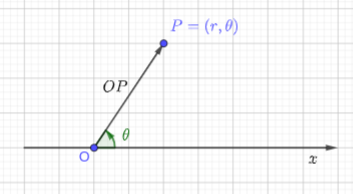
\includegraphics[width=0.6\textwidth]{cap_osc/dados/fig_osc_scp/fig}
  \caption{Sistema de coordenadas polares.}
  \label{fig:osc_scp}
\end{figure}

Neste sistema, um ponto $P$ de coordenadas polares ${\color{blue}P=(r, \theta)}$ é tal que ${\color{blue}|OP| = r}$ (i.e. a distância do polo ao ponto é $r$) e ${\color{blue}\theta}$ é o ângulo de $Ox$ com $OP$, medido positivamente no sentido anti-horário.

\begin{ex}
  Na Figura \ref{fig:ex_osc_scp}, temos a representação dos pontos ${\color{blue}P=(2\sqrt{2}, \frac{\pi}{4})}$, ${\color{red}A=(2, \frac{2\pi}{3})}$ e ${\color{orange}B=(\sqrt{2}, \frac{5\pi}{4})}$ no sistema de coordenadas polares.

\begin{figure}[H]
  \centering
  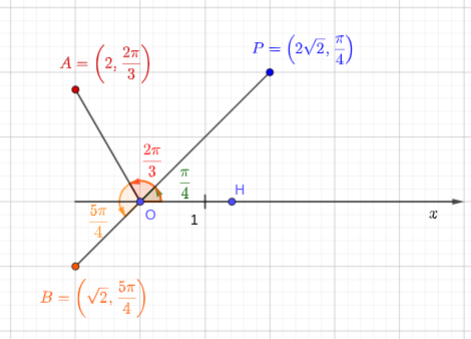
\includegraphics[width=0.6\textwidth]{cap_osc/dados/fig_ex_osc_scp/fig}
  \caption{Sistema de coordenadas polares.}
  \label{fig:ex_osc_scp}
\end{figure}  
\end{ex}

\begin{obs}
  Por convenção, as coordenadas polares $(r, \pi + \theta) = (-r, \theta)$, $r>0$. Por exemplo, $B=(\sqrt{2}, \frac{5\pi}{4}) = (-\sqrt{2}, \frac{\pi}{4})$. Veja na Figura \ref{fig:ex_osc_scp}.
\end{obs}

\subsection{Coordenadas cartesianas x polares}

Aqui, vamos estudar como podemos converter as coordenadas de um ponto $P$ de coordenadas cartesianas para coordenadas polares e vice-versa. Vamos denotar as coordenadas cartesianas do ponto $P$ por $P=(x_P, y_P)$ e suas coordenadas polares por $P=(r, \theta)$. Veja a Figura \ref{fig:osc_ccxcp}.

\begin{figure}[H]
  \centering
  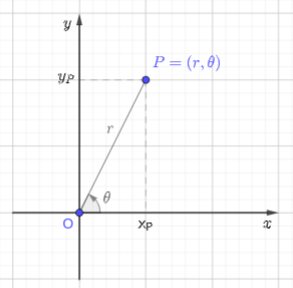
\includegraphics[width=0.5\textwidth]{cap_osc/dados/fig_osc_ccxcp/fig}
  \caption{Sistema de coordenadas polares.}
  \label{fig:osc_ccxcp}
\end{figure}  

Na Figura \ref{fig:osc_ccxcp}, vamos nos concentrar no triângulo retângulo de vértices $O$, $(x_P, 0)$ e $P$. Das relações trigonométricas e do teorema de Pitágoras, temos que
\begin{gather}
  \cos\theta = \frac{x_P}{r} \\
  \sen\theta = \frac{y_P}{r} \\
  r^2 = x_P^2 + y_P^2 \\
  \tg\theta = \frac{y_P}{x_P}
\end{gather}
ou, equivalentemente,
\begin{gather}
  {\color{blue}x_P = r\cos\theta} \\
  {\color{blue}y_P = r\sen\theta} \\
  {\color{blue}r = \sqrt{x_P^2 + y_P^2 }} \\
  {\color{blue}\theta = \arc\tg\left(\frac{y_P}{x_P}\right)}
\end{gather}

\begin{ex}
  Vejamos os seguintes casos:
  \begin{enumerate}
  \item[a)] Conversão de $P=(2\sqrt{2}, \frac{\pi}{4})$ em coordenadas polares para coordenadas cartesianas.

    No caso de $P=(2\sqrt{2}, \frac{\pi}{4}$ temos $r=2\sqrt{2}$ e $\theta = \frac{\pi}{4}$. Desta forma, as coordenadas cartesianas de $P=(x,y)$ são dadas por
    \begin{align}
      x &= r\cos\theta \\
        &= 2\sqrt{2}\cos\frac{\pi}{4}\\
        &= 2\sqrt{2}\cdot \frac{\sqrt{2}}{2}\\
        &= 2\\
      ~&~\nonumber\\
      y &= r\sen\theta\\
        &= 2\sqrt{2}\sen\frac{\pi}{4}\\
        &= 2\sqrt{2}\cdot\frac{\sqrt{2}}{2}\\
        &= 2
    \end{align}
    Logo, $P=(2,2)$ em coordenadas cartesianas. Veja a Figura \ref{fig:ex_osc_scp}.

  \item[b)] Conversão de $B=(-\sqrt{3}, -1)$ de coordenadas cartesianas para coordenadas polares. Neste caso, temos $x=-\sqrt{3}$ e $y=-1$ e
    \begin{align}
      r &= \sqrt{x^2 + y^2} \\
        &= \sqrt{(-\sqrt{3})^2 + (-1)^2}\\
        &= \sqrt{4} \\
        &= 2\\
      ~&~\nonumber\\
      \theta &= \arc\tg\left(\frac{y}{x}\right)\\
        &= \arc\tg\left(\frac{-1}{-\sqrt{3}}\right)\\
        &= \arc\tg\left(\frac{\sqrt{3}}{3}\right)\\
        &= \frac{7\pi}{6}.
    \end{align}
    Desta forma, temos que $P=(2, \frac{7\pi}{6})$ em coordenadas polares. Ou, equivalentemente, $P=(-2, \frac{\pi}{6})$.
  \end{enumerate}
\end{ex}

\subsubsection{Equação de reta que passa pela origem}

Em coordenadas polares, uma reta que passa pela origem e tem ângulo de declividade $\theta_0$ tem equação
\begin{equation}
  \theta = \theta_0,
\end{equation}
com $r\in\mathbb{R}$.

\begin{ex}
  Seja a reta $y=x$ em coordenadas cartesianas. Em coordenadas polares, a equação desta reta é
  \begin{equation}
    \theta = \frac{\pi}{4}.
  \end{equation}
\end{ex}

\subsubsection{Equação de circunferência com centro na origem}

Em coordenadas polares, a circunferência com centro na origem e raio $r_0$ tem equação
\begin{equation}
  r = r_0.
\end{equation}

\begin{ex}
  Seja a circunferência $x^2 + y^2 = 4$ em coordenadas cartesianas. Em coordenadas polares, a equação desta circunferência é
  \begin{equation}
    r = 2.
  \end{equation}
\end{ex}

\subsection{Exercícios resolvidos}

\begin{exeresol}
  Obtenha duas representações em coordenadas polares do ponto $A=(-1,0)$ dado em coordenadas cartesianas.
\end{exeresol}
\begin{resol}
  O ponto $A=(-1, 0)$ tem coordenadas cartesianas $x=-1$ e $y=0$. Para converter em coordenadas polares $A=(r, \theta)$, podemos usar
  \begin{align}
    r^2 &= x^2 + y^2 \\
    r^2  &= 1^2 + 0^2 \\
    r  &= \pm 1
  \end{align}
  e
  \begin{align}
    \theta &= \arc\tg\left(\frac{y}{x}\right) \\
           &= \arc\tg\left(0\right) \\
           &= \pi\text{ ou }0. 
  \end{align}
  Ou seja, em coordenadas polares, temos as representações $A=(1, \pi)$ ou $A=(-1,0)$.
\end{resol}

\begin{exeresol}
  Obtenha a representação em coordenadas cartesianas do ponto $B=(2, \frac{\pi}{2})$ dado em coordenadas polares.
\end{exeresol}
\begin{resol}
  O ponto $B=(2, \frac{\pi}{2})$ tem coordenadas polares $r=2$ e $\theta=\frac{\pi}{2}$. Para converter em coordenadas cartesianas $B=(x, y)$, podemos usar
  \begin{align}
    x &= r\cos\theta \\
      &= 2\cos\frac{\pi}{2} \\
      &= 0
  \end{align}
  e
  \begin{align}
    y &= r\sen\theta \\
      &= 2\sen\frac{\pi}{2} \\
      &= 2 
  \end{align}
  Ou seja, em coordenadas cartesianas, temos a representação $B=(0, 2)$.
\end{resol}

\subsection*{Exercícios}

\begin{exer}
  Obtenha uma representação em coordenadas polares dos seguintes pontos dados em coordenadas cartesianas:
  \begin{enumerate}[a)]
  \item $A=(-3, 3)$
  \item $B=(\frac{3}{2}, \frac{\sqrt{3}}{2})$
  \item $C=(\frac{3}{2}, -\frac{\sqrt{3}}{2})$
  \end{enumerate}
\end{exer}
\begin{resp}
  a) $A=(3\sqrt{2}, \frac{3\pi}{4})$; b) $B = (\sqrt{3}, \frac{\pi}{6})$; c) $C=(\sqrt{3}, \frac{11\pi}{6})$
\end{resp}

\begin{exer}
  Obtenha uma representação em coordenadas cartesianas dos seguintes pontos dados em coordenadas polares:
  \begin{enumerate}[a)]
  \item $A=(2, \frac{\pi}{6})$
  \item $B=(1, \frac{5 \pi}{6})$
  \item $C=(-2, \frac{3\pi}{4})$
  \end{enumerate}
\end{exer}
\begin{resp}
  a) $A=(\sqrt{3}, 1)$; b) $B = (-\frac{\sqrt{3}}{2}, \frac{1}{2})$; c) $C=(\sqrt{2}, -\sqrt{2})$
\end{resp}

\begin{exer}
  Considere a reta de equação $x = 0$ em coordenadas cartesianas. Escreva a equação desta reta em coordenadas polares.
\end{exer}
\begin{resp}
  $\theta = \frac{\pi}{2}$
\end{resp}

\begin{exer}
  Considere a reta de equação $\theta = \frac{3\pi}{4}$ em coordenadas polares. Escreva a equação desta reta em coordenadas cartesianas.
\end{exer}
\begin{resp}
  $y = -x$
\end{resp}

\begin{exer}
  Considere a circunferência de equação $x^2 + y^2 = 1$ em coordenadas cartesianas. Escreva a equação desta circunferência em coordenadas polares.
\end{exer}
\begin{resp}
  $r = 1$
\end{resp}

\begin{exer}
  Considere a circunferência de equação $r = \sqrt{2}$ em coordenadas polares. Escreva a equação desta circunferência em coordenadas cartesianas.
\end{exer}
\begin{resp}
  $x^2 + y^2 = 2$
\end{resp}

%Este trabalho está licenciado sob a Licença Atribuição-CompartilhaIgual 4.0 Internacional Creative Commons. Para visualizar uma cópia desta licença, visite http://creativecommons.org/licenses/by-sa/4.0/deed.pt_BR ou mande uma carta para Creative Commons, PO Box 1866, Mountain View, CA 94042, USA.

\chapter{Cônicas}\label{cap_conicas}
\thispagestyle{fancy}

Neste capítulo, fazemos um estudo introdutório sobre cônicas no plano cartesiano. Mais precisamente, vamos estudar as equações de elipses, hipérboles e parábolas.

\section{Elipse}\label{cap_conicas_sec_elipse}

Sejam $F_1$, $F_2$ pontos sobre um plano $\pi$, $c = \frac{1}{2}|F_1F_2|$ e $a > c$. Chama-se \emph{elipse} de \emph{focos} $F_1$ e $F_2$ ao conjunto de pontos $P$ tais que
\begin{equation}
  {\color{blue}|PF_1| + |PF_2| = 2a}.
\end{equation}
Veja a Figura \ref{fig:elipse}.

\begin{figure}[H]
  \centering
  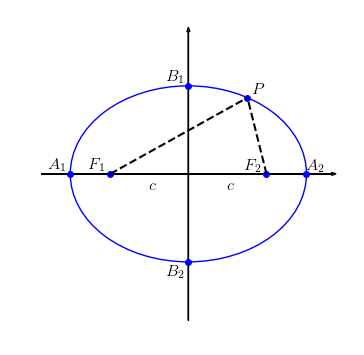
\includegraphics[width=0.7\textwidth]{./cap_conicas/dados/fig_elipse/fig_elipse}
  \caption{Ilustração de uma elipse de focos $F_1$ e $F_2$.}
  \label{fig:elipse}
\end{figure}

Dada uma tal elipse, identificamos $2c=|F_1F_2|$ como a \emph{distância focal}. Os pontos $A_1$ e $A_2$ de interseção da elipse com a reta que passa pelos focos são chamados de \emph{vértices} da elipse. O segmento $A_1A_2$ é chamado de \emph{eixo maior} da elipse. Observamos que
\begin{equation}
  |A_1A_2| = 2a.
\end{equation}
O ponto médio do segmento $F_1F_2$ é chamado de \emph{centro} da elipse. Sejam $B_1$ e $B_2$ os pontos de interseção da elipse com a reta que passa pelo centro da elipse e é perpendicular ao segmento $A_1A_2$. Assim sendo, o segmento $B_1B_2$ é chamado de \emph{eixo menor} da elipse. Vamos denotar
\begin{equation}
  2b = |B_1B_2|.
\end{equation}

Chamamos de \emph{excentricidade} da elipse o número
\begin{equation}
  e = \frac{c}{a}.
\end{equation}
Notemos que $0 \leq e < 1$. Para $e=0$, temos $c=0$ e, portanto $F_1=F_2$. Neste caso, a elipse é a circunferência de centro em $F_1$ (ou $F_2$) e diâmetro $2a$. No que $e$ tende a $1$, a elipse tende ao segmento $A_1A_2$.

Por fim, notamos que o triângulo $B_1OF_2$ é retângulo, $|OF_2|=c$, $|F_2B_1|=a$ e $|OB_1|=b$. Do teorema de Pitágoras segue
\begin{equation}\label{eq:elipse_obs}
  b^2 + c^2 = a^2.
\end{equation}

\subsection{Equação reduzida da elipse}

Consideremos o sistema de coordenadas cartesianas. Sejam $F_1=(-c,0)$ e $F_2=(c,0)$, $c\geq 0$, os focos de uma dada elipse (veja a Figura \ref{fig:elipse}).  Se $P=(x,y)$ é um ponto da elipse, então
\begin{equation}
  |PF_1| + |PF_2| = 2a.
\end{equation}
Como
\begin{align}
  |PF_1| &= \sqrt{(x+c)^2 + y^2}, \\
  |PF_2| &= \sqrt{(x-c)^2 + y^2},
\end{align}
temos
\begin{equation}
  \sqrt{(x+c)^2 + y^2} + \sqrt{(x-c)^2 + y^2} = 2a,
\end{equation}
ou, equivalentemente,
\begin{equation}
  \sqrt{(x+c)^2 + y^2} = 2a - \sqrt{(x-c)^2 + y^2}.
\end{equation}
Elevando ao quadrado, obtemos
\begin{equation}
  (x+c)^2 + y^2 = 4a^2 - 4a\sqrt{(x-c)^2+y^2} + (x-c)^2+y^2.
\end{equation}
Por cancelamento e rearranjo dos termos, obtemos
\begin{equation}
  a\sqrt{(x-c)^2+y^2}=a^2-cx.
\end{equation}
Elevando novamente ao quadrado, temos
\begin{equation}
  a^2(x-c)^2+a^2y^2=a^4-2a^2cx+c^2x^2,
\end{equation}
donde
\begin{equation}
  a^2x^2 -2a^2cx + a^2c^2 + a^2y^2= a^4 -2a^2cx + c^2x^2.
\end{equation}
Por cancelamento e rearranjo dos termos, obtemos
\begin{equation}
  x^2(a^2 - c^2) + a^2y^2 = a^2(a^2 - c^2).
\end{equation}
Como $a>c$, dividimos por $a^2-c^2$  e depois por $a^2$ para obtemos
\begin{equation}
  \frac{x^2}{a^2} + \frac{y^2}{a^2-c^2} = 1.
\end{equation}
Por fim, da equação \eqref{eq:elipse_obs}, temos $a^2-c^2 = b^2$, o que nos leva  a \emph{equação reduzida da elipse}
\begin{equation}
  {\color{blue}\frac{x^2}{a^2} + \frac{y^2}{b^2} = 1}.
\end{equation}

\begin{ex}
  A Figura \ref{fig:elipse_ex} é um esboço do gráfico da elipse de equação reduzida
  \begin{equation}
    \frac{x^2}{25} + \frac{y^2}{16} = 1.
  \end{equation}

  \begin{figure}[H]
    \centering
    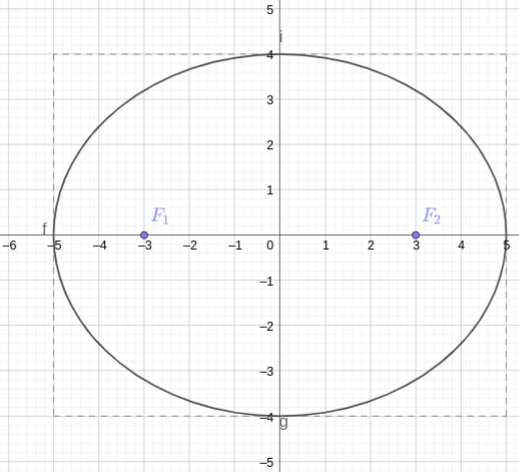
\includegraphics[width=0.5\textwidth]{cap_conicas/dados/fig_ex_elipse/fig}
    \caption{Esboço do gráfico da elipse $\displaystyle\frac{x^2}{25}-\frac{y^2}{16}=1$.}
    \label{fig:elipse_ex}
  \end{figure}
\end{ex}

\subsection*{Exercícios resolvidos}

\begin{exeresol}
  Determine a equação reduzida da elipse de focos $F_1=(-3,0)$, $F_2=(3,0)$ e vértices $A_1=(-5,0)$ e $A_2=(5,0)$.
\end{exeresol}
\begin{resol}
  A equação reduzida tem a forma
  \begin{equation}
    \frac{x^2}{a^2} + \frac{y^2}{b^2} = 1,
  \end{equation}
  onde
  \begin{equation}
    b^2 + c^2 = a^2.
  \end{equation}
  Dos focos temos $c=3$ e dos vértices temos $a=5$. Logo,
  \begin{align}
    b^2 &=  a^2 - c^2 \\
        &= 5^2 - 3^2 \\
        &= 25 - 9 \\
        &= 16.
  \end{align}
  Concluímos que a elipse em questão tem equação
  \begin{equation}
    \frac{x^2}{25} - \frac{y^2}{16} = 1.
  \end{equation}
\end{resol}

\begin{exeresol}
  Determine os focos da elipse de equação
  \begin{equation}
    \frac{x^2}{16} + \frac{y^2}{25} = 1.
  \end{equation}
\end{exeresol}
\begin{resol}
  Começamos lembrando que os focos de uma elipse estão localizados sobre seu eixo maior. No caso deste exercício, temos $a=4$ e $b=5$, logo o eixo maior é $B_1B_2$, na mesma direção do eixo das ordenadas $Oy$. Do triângulo retângulo $OA_2F_1$ temos
  \begin{equation}
    b^2 = a^2 + c^2,
  \end{equation}
  veja a Figura \ref{fig:elipse_exeresol1}.

  \begin{figure}[H]
    \centering
    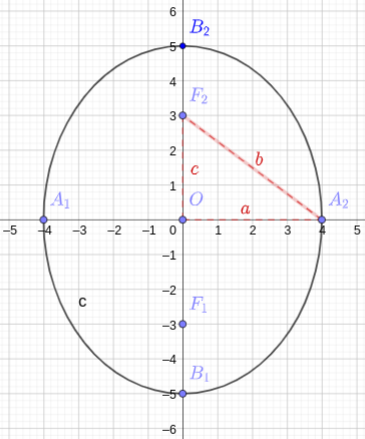
\includegraphics[width=0.5\textwidth]{cap_conicas/dados/fig_elipse_exeresol1/fig}
    \caption{Esboço do gráfico de uma elipse com eixo maior sobre o eixo das ordenadas $Oy$.}
    \label{fig:elipse_exeresol1}
  \end{figure}

  Daí, temos
  \begin{align}
    c^2 &= b^2 - a^2 \\
        &= 25 - 16 \\
        &= 9 \\
    c &= 3.
  \end{align}
  Concluímos que os focos são $F_1=(0,-3)$ e $F_2=(0,3)$.
\end{resol}

\subsection*{Exercícios}

\begin{exer}
  Faça um esboço da elipse de equação reduzida
  \begin{equation}
    \frac{x^2}{9} + \frac{y^2}{4} = 1.
  \end{equation}
\end{exer}
\begin{resp}
  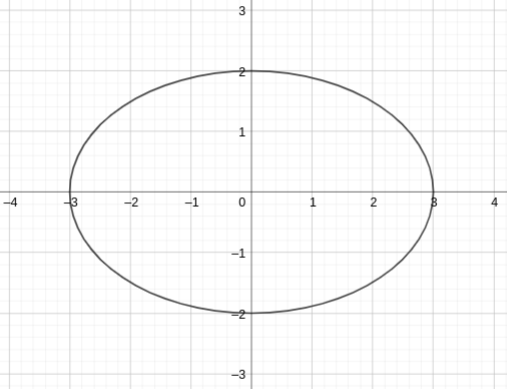
\includegraphics[width=0.5\textwidth]{cap_conicas/dados/fig_elipse_exer_ox/fig}
\end{resp}

\begin{exer}
  Faça um esboço da elipse de equação reduzida
  \begin{equation}
    \frac{x^2}{4} + \frac{y^2}{9} = 1.
  \end{equation}
\end{exer}
\begin{resp}
  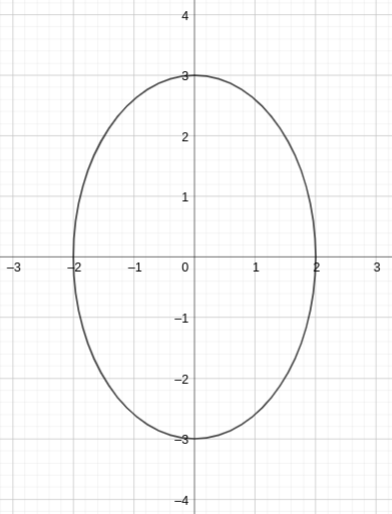
\includegraphics[width=0.4\textwidth]{cap_conicas/dados/fig_elipse_exer_oy/fig}
\end{resp}

\begin{exer}
  Determine os vértices (sobre o eixo maior) das seguintes elipses:
  \begin{enumerate}[a)]
  \item $\displaystyle \frac{x^2}{9} + \frac{y^2}{4} = 1$
  \item $\displaystyle x^2 + \frac{y^2}{16} = 1$
  \end{enumerate}
\end{exer}
\begin{resp}
  a)~$(-3, 0)$, $(3, 0)$; b)~$(0, -4)$, $(0, 4)$
\end{resp}

\begin{exer}
  Determine os focos das seguintes elipses:
  \begin{enumerate}[a)]
  \item $\displaystyle \frac{x^2}{9} + \frac{y^2}{4} = 1$
  \item $\displaystyle x^2 + \frac{y^2}{16} = 1$
  \end{enumerate}
\end{exer}
\begin{resp}
  a)~$(-\sqrt{5}, 0)$, $(\sqrt{5}, 0)$; b)~$(0, \sqrt{3})$, $(0, \sqrt{3})$
\end{resp}

\begin{exer}
  Forneça a equação reduzida da elipse de focos $F_1=(-1, 0)$, $F_2=(1, 0)$ e vértices $A_1=(-\sqrt{2}, 0)$, $A_2=(\sqrt{2}, 0)$.
\end{exer}
\begin{resp}
  $\displaystyle\frac{x^2}{2}+y^2=1$
\end{resp}

\begin{exer}
  Forneça a equação reduzida da elipse de focos $F_1=(0, -2)$, $F_2=(0, 2)$ e vértices $B_1=(0, -\sqrt{5})$, $B_2=(0, \sqrt{5})$.
\end{exer}
\begin{resp}
  $\displaystyle x^2+\frac{y^2}{5}=1$
\end{resp}

\section{Hipérbole}\label{cap_conicas_sec_hiperbole}

Sejam $F_1$ e $F_2$ pontos sobre um plano $\pi$. Sejam, também, $c$ tal que $|F_1F_2|=2c$ e $a<c$. O lugar geométrico dos pontos $P$ tais que
\begin{equation}
  {\color{blue}||PF_1|-|PF_2||=2a},
\end{equation}
chama-se \emph{hipérbole}. Veja Figura \ref{fig:hiperbole}.

\begin{figure}[H]
  \centering
  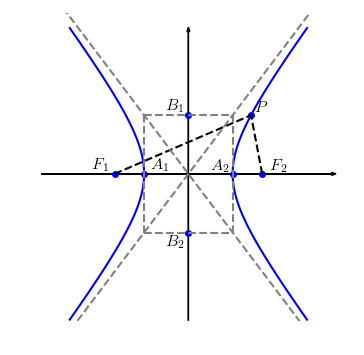
\includegraphics[width=0.7\textwidth]{./cap_conicas/dados/fig_hiperbole/fig_hiperbole}
  \caption{Ilustração de uma hipérbole de focos $F_1$ e $F_2$.}
  \label{fig:hiperbole}
\end{figure}

Os pontos $F_1$ e $F_2$ são chamados de \emph{focos} da hipérbole e $2c = |F_1F_2|$ é chamada de \emph{distância focal}. O ponto médio entre os pontos $F_1$ e $F_2$ é chamado de centro da hipérbole. São chamados \emph{vértices} da hipérbole os pontos $A_1$ e $A_2$, sendo que o segmento $A_1A_2$ é chamado de \emph{eixo real} (ou transverso) da hipérbole. O comprimento deste eixo é $|A_1A_2|=2a$.

Sejam $B_1$ e $B_2$ pontos $c$ distantes de $A_1$ e $A_2$ e pertencentes a reta que passa pelo centro da hipérbole e é perpendicular ao seu eixo real. O segmento $B_1B_2$ é chamado de \emph{eixo imaginário} (transverso ou conjugado). Denotando $2b=|B_1B_2|$, temos do triângulo retângulo $B_1OA_1$ que
\begin{equation}
  {\color{blue}c^2 = a^2 + b^2}.
\end{equation}

\subsection{Equação reduzida da hipérbole}

Assumimos um sistema de coordenadas cujo centro coincida com o centro de uma dada hipérbole e o eixo das abscissas seja coincidente com o eixo real da hipérbole. Desta forma, temos $F_1 = (-c,0)$ e $F_2 = (c,0)$. Então, $P=(x,y)$ é um ponto da hipérbole quando
\begin{equation}
  ||PF_1|-|PF_2|| = 2a.
\end{equation}
Daí, segue que
\begin{gather}
  |PF_1|-|PF_2| = \pm 2a \\
  \sqrt{(x+c)^2+y^2}-\sqrt{(x-c)^2+y^2} =\pm 2a\\
  \sqrt{(x+c)^2+y^2} = \pm 2a + \sqrt{(x-c)^2+y^2}
\end{gather}
Elevando ao quadrado ambos os lados desta última equação, obtemos
\begin{align}
  (x+c)^2+y^2 &= 4a^2 \pm 4a\sqrt{(x-c)^2+y^2} \\
              &+ (x-c)^2+y^2
\end{align}
ou, equivalentemente,
\begin{align}
  x^2+2cx+c^2+y^2 &= 4a^2\pm4a\sqrt{(x-c)^2+y^2}\\
                  &+x^2-2cx+c^2+y^2
\end{align}
Simplificando e rearranjando os termos, temos
\begin{equation}
  cx - a^2 = \pm a\sqrt{(x-c)^2+y^2}).
\end{equation}
Elevando novamente ao quadrado, obtemos
\begin{equation}
  c^2x^2 - 2a^2cx + a^4 = a^2x^2 - 2a^2cx + a^2c^2 + a^2y^2.
\end{equation}
Simplificando e rearranjando os termos, obtemos
\begin{equation}
  (c^2-a^2)x^2 - a^2y^2 = a^2(c^2-a^2).
\end{equation}
Lembrando que $c^2 = a^2 + b^2$, temos
\begin{equation}
  b^2x^2 - a^2y^2 = a^2b^2.
\end{equation}
Dividindo por $a^2b^2$, obtemos
\begin{equation}\label{eq:hiperbole_red}
  {\color{blue}\frac{x^2}{a^2} - \frac{y^2}{b^2} = 1},
\end{equation}
a qual é chamada de \emph{equação reduzida da hipérbole}.

\begin{ex}
  A Figura \ref{fig:ex_hiperbole} é um esboço do gráfico da hipérbole de equação reduzida
  \begin{equation}
    \frac{x^2}{16} - \frac{y^2}{9} = 1.
  \end{equation}

  \begin{figure}[H]
    \centering
    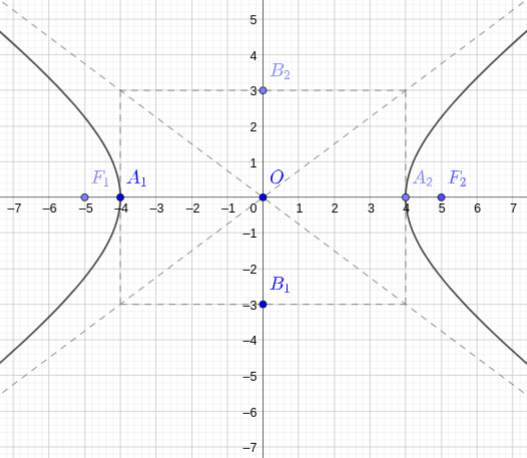
\includegraphics[width=0.7\textwidth]{cap_conicas/dados/fig_ex_hiperbole/fig}
    \caption{Esboço do gráfico da hipérbole de equação $\displaystyle\frac{x^2}{16}-\frac{y^2}{9}=1$.}
    \label{fig:ex_hiperbole}
  \end{figure}  
\end{ex}

\subsection*{Exercícios resolvidos}

\begin{exeresol}
  Obtenha a equação reduzida da hipérbole centrada na origem e de eixo real $|A_1A_2|=8$ e eixo imaginário $|B_1B_2|=4$.
\end{exeresol}
\begin{resol}
  A equação reduzida de uma hipérbole centrada na origem tem a forma
  \begin{equation}
    \frac{x^2}{a^2} - \frac{y^2}{b^2} = 1,
  \end{equation}
  onde $2a = |A_1A_2|$ e $2b=|B_1B_2|$. No caso deste exercício, temos
  \begin{equation}
    2a = 8 \Rightarrow a = 4
  \end{equation}
  e
  \begin{equation}
    2b = 4 \Rightarrow b = 2
  \end{equation}
  Logo, a equação buscada é
  \begin{equation}
    \frac{x^2}{4^2} - \frac{y^2}{2^2} = 1
  \end{equation}
  ou, equivalentemente,
  \begin{equation}
    \frac{x^2}{16} - \frac{y^2}{4} = 1.
  \end{equation}  
\end{resol}

\begin{exeresol}
  Faça o esboço da hipérbole de equação reduzida
  \begin{equation}
    \frac{y^2}{16} - \frac{x^2}{9} = 1.
  \end{equation}
\end{exeresol}
\begin{resol}
  Observe que nesta equação, o termo contendo $x$ tem sinal negativo e o termo contendo $y$ tem sinal positivo (compare com \eqref{eq:hiperbole_red}). Isto nos indica que o eixo real desta hipérbole está na direção das ordenadas $Oy$ e, consequentemente, o eixo imaginário na direção das abscissas $Ox$.

  Da equação, temos $a^2 = 9$ e $b^2=16$, donde $a=3$ e $b=4$. Neste caso, os vértices que definem o eixo real são $A_1=(0, -b)=(0, -4)$ e $A_2=(0, b)=(0, 4)$. Os focos $F_1=(0, -c)$ e $F_2=(0, c)$ são tais que
  \begin{align}
    c^2 &= a^2 + b^2 \\
        &= 9 + 16 \\a
        &= 25 \\
    c &= 5.
  \end{align}
  Com estas informações, traçamos o esboço dado na Figura \ref{fig:hiperbole_exeresol_oy}.

  \begin{figure}[H]
    \centering
    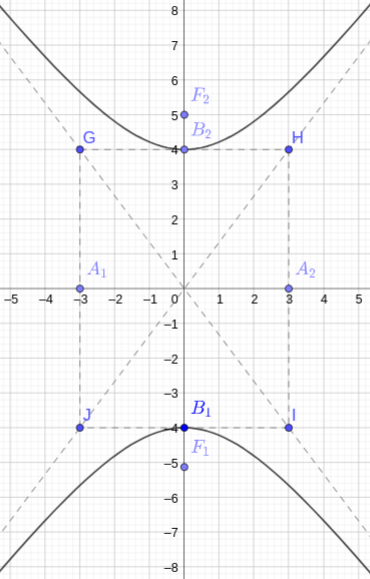
\includegraphics[width=0.5\textwidth]{cap_conicas/dados/fig_hiperbole_exeresol_oy/fig}
    \caption{Esboço do gráfico da hipérbole de equação $\displaystyle\frac{y^2}{16}-\frac{x^2}{9}=1$.}
    \label{fig:hiperbole_exeresol_oy}
  \end{figure}   
\end{resol}

\begin{exeresol}
  Mostre que uma hipérbole de equação reduzida
  \begin{equation}
    \frac{x^2}{a^2} - \frac{y^2}{b^2} = 1
  \end{equation}
  tem assíntotas
  \begin{equation}
    y = \pm \frac{b}{a}x.
  \end{equation}
\end{exeresol}
\begin{resol}
  De fato, ao isolarmos $y$ na equação reduzida, obtemos
  \begin{equation}
    y = \pm\sqrt{\frac{b^2}{a^2}x^2 - b^2}
  \end{equation}
  Logo, para $x\to \infty$, temos
  \begin{gather}
    y\to \pm\sqrt{\frac{b^2}{a^2}x^2} \\
    y\to \pm\sqrt{\frac{b^2}{a^2}}\sqrt{x^2}\\
    y\to \pm\frac{b}{a}x
  \end{gather}
  De forma análoga, quando $x\to -\infty$, temos
  \begin{gather}
    y\to \pm\sqrt{\frac{b^2}{a^2}x^2} \\
    y\to \pm\sqrt{\frac{b^2}{a^2}}\sqrt{x^2}\\
    y\to \mp\frac{b}{a}x
  \end{gather}
  Ambos os resultados mostram que $\displaystyle y=\pm\frac{b}{a}x$ são assíntotas da hipérbole.
\end{resol}

\subsection*{Exercícios}

\begin{exeresol}
  Faça o esboço da hipérbole de equação reduzida
  \begin{equation}
    \frac{x^2}{9} - \frac{y^2}{4} = 1
  \end{equation}
\end{exeresol}
\begin{resp}
  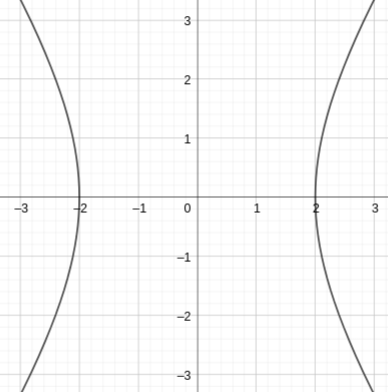
\includegraphics[width=0.5\textwidth]{cap_conicas/dados/fig_hiperbole_exer_ox/fig}
\end{resp}

\begin{exeresol}
  Faça o esboço da hipérbole de equação reduzida
  \begin{equation}
    \frac{y^2}{9} - \frac{x^2}{4} = 1
  \end{equation}
\end{exeresol}
\begin{resp}
  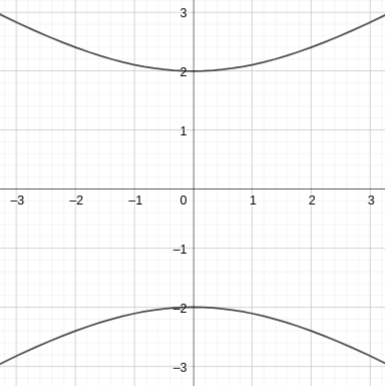
\includegraphics[width=0.5\textwidth]{cap_conicas/dados/fig_hiperbole_exer_oy/fig}
\end{resp}

\begin{exer}
  Determine os vértices do eixo real das seguintes hipérboles:
  \begin{enumerate}[a)]
  \item $\displaystyle \frac{x^2}{9} - \frac{y^2}{4} = 1$
  \item $\displaystyle y^2 - \frac{x^2}{16} = 1$
  \end{enumerate}
\end{exer}
\begin{resp}
  a)~$A_1=(-3,0)$, $A_2=(3,0)$; b)~$B_1=(0, -1)$, $B_2=(0, 1)$
\end{resp}

\begin{exer}
  Determine os focos das seguintes hipérboles:
  \begin{enumerate}[a)]
  \item $\displaystyle \frac{x^2}{9} - \frac{y^2}{4} = 1$
  \item $\displaystyle y^2 - \frac{x^2}{16} = 1$
  \end{enumerate}
\end{exer}
\begin{resp}
  a)~$F_1=(-\sqrt{13}, 0)$, $F_2=(\sqrt{13}, 0)$; b)~$F_1=(0, -\sqrt{17})$, $F_2=(0, \sqrt{17})$
\end{resp}

\begin{exer}
  Forneça a equação reduzida da hipérbole de focos $F_1=(-2, 0)$, $F_2=(2, 0)$ e de vértices do eixo real $A_1=(-1, 0)$ e $A_2=(1, 0)$.
\end{exer}
\begin{resp}
  $\displaystyle x^2 - \frac{y^2}{3} = 1$
\end{resp}

\begin{exer}
  Forneça a equação reduzida da hipérbole de distância focal $|F_1F_2|=2\sqrt{6}$ e de vértices do eixo imaginário $A_1=(-2, 0)$ e $A_2=(2, 0)$.
\end{exer}
\begin{resp}
  $\displaystyle \frac{y^2}{2} - \frac{x^2}{4} = 1$
\end{resp}

\section{Parábola}\label{cap_conicas_sec_parabola}

Em um plano, consideramos uma reta $d$ e um ponto $F$ não pertencente a $d$. Chamamos de \emph{parábola} o conjunto de pontos $P$ do plano que são equidistantes de $F$ e de $d$, i.e.
\begin{equation}
  {\color{blue}\dist(P, F) = \dist(P, d)}.
\end{equation}
Veja a Figura \ref{fig:parabola}.

\begin{figure}[H]
  \centering
  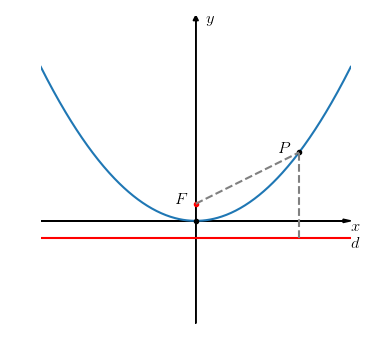
\includegraphics[width=0.7\textwidth]{./cap_conicas/dados/fig_parabola/fig_parabola}
  \caption{Ilustração de uma parábola.}
  \label{fig:parabola}
\end{figure}

O ponto $F$ é chamado de \emph{foco} da parábola. A reta $d$ é chamada de \emph{diretriz} da parábola. A reta perpendicular a $d$ e que passa pelo ponto $F$ é chamada de \emph{eixo} da parábola. O ponto $V$ de interseção entre a parábola e seu eixo é chamado de \emph{vértice} da parábola.

\subsection{Equação reduzida de uma parábola}

Tomamos o sistema cartesiano de coordenadas com origem no vértice da parábola e eixo das abscissas paralelo à diretriz. Seja $p$ tal que
\begin{equation}
  F = (0, p/2).
\end{equation}
Logo, a diretriz tem equação $y = -p/2$. Da definição de parábola, $P=(x,y)$ pertence a parábola quando
\begin{equation}
  \dist(P, F) = \dist(P, d).
\end{equation}
Segue que
\begin{equation}
  \sqrt{x^2+\left(y-\frac{p}{2}\right)^2} = y+\frac{p}{2}.
\end{equation}
Elevando ao quadrado e expandindo, obtemos
\begin{equation}
  x^2 + y^2-py+\frac{p^2}{4} = y^2 + py + \frac{p^2}{4}.
\end{equation}
Cancelando e rearranjando termos, obtemos
\begin{equation}
  {\color{blue}x^2 = 2py},
\end{equation}
a chamada \emph{equação reduzida da parábola}.

\begin{ex}
  A Figura \ref{fig:parabola_ex} é um esboço do gráfica da parábola de equação reduzida
  \begin{equation}
    x^2 = 4y.
  \end{equation}

  \begin{figure}[H]
    \centering
    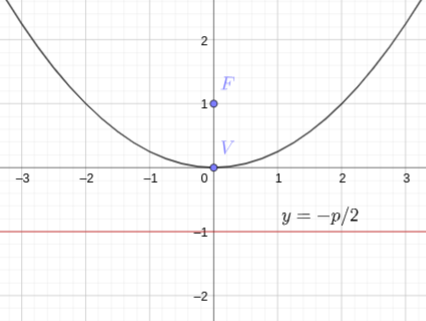
\includegraphics[width=0.6\textwidth]{cap_conicas/dados/fig_parabola_ex/fig}
    \caption{Esboço do gráfico da parábola de equação $y^2 = 4x$.}
    \label{fig:parabola_ex}
  \end{figure}
\end{ex}

\begin{obs}
  Uma parábola com vértice na origem do sistema cartesiano e foco $F=(p/2, 0)$, tem equação reduzida
  \begin{equation}
    y^2 = 2px.
  \end{equation}
\end{obs}

\subsection*{Exercícios resolvidos}

\begin{exeresol}
  Determine a equação reduzida da parábola de diretriz $y=2$ e vértice na origem do sistema cartesiano. Por fim, faça o esboço de seu gráfico.
\end{exeresol}
\begin{resol}
  Uma parábola de equação reduzida
  \begin{equation}
    x^2 = 2py
  \end{equation}
  tem diretriz $\displaystyle y=-\frac{p}{2}$. Logo, sabendo que a diretriz é $y=2$, temos $p = -4$. Então, concluímos que a equação reduzida da parábola é
  \begin{equation}
    x^2 = -8y
  \end{equation}
  A Figura \ref{fig:parabola_exeresol_yp} é o esboço do gráfico desta parábola.

  \begin{figure}[H]
    \centering
    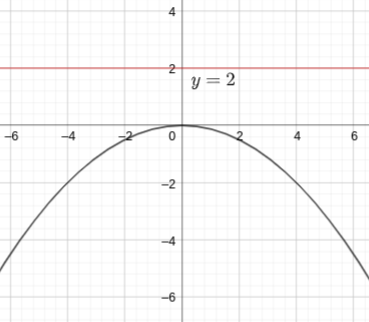
\includegraphics[width=0.6\textwidth]{cap_conicas/dados/fig_parabola_exeresol_yp/fig}
    \caption{Esboço do gráfico da parábola de equação $y^2 = -8x$.}
    \label{fig:parabola_exeresol_yp}
  \end{figure}  
\end{resol}

\begin{exeresol}
  Determine a equação reduzida da parábola de diretriz $x=2$ e vértice na origem do sistema cartesiano. Por fim, faça o esboço de seu gráfico.
\end{exeresol}
\begin{resol}
  Uma parábola de equação reduzida
  \begin{equation}
    y^2 = 2px
  \end{equation}
  tem diretriz $\displaystyle x=-\frac{p}{2}$. Logo, sabendo que a diretriz é $x=2$, temos $p = -4$. Então, concluímos que a equação reduzida da parábola é
  \begin{equation}
    y^2 = -8x
  \end{equation}
  A Figura \ref{fig:parabola_exeresol_xp} é o esboço do gráfico desta parábola.

  \begin{figure}[H]
    \centering
    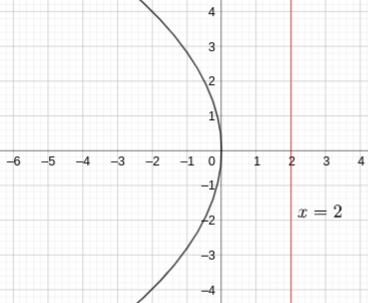
\includegraphics[width=0.6\textwidth]{cap_conicas/dados/fig_parabola_exeresol_xp/fig}
    \caption{Esboço do gráfico da parábola de equação $y^2 = -8x$.}
    \label{fig:parabola_exeresol_xp}
  \end{figure}  
\end{resol}

\subsection*{Exercícios}

\begin{exer}
  Faça o esboço do gráfico da parábola de equação reduzida
  \begin{equation}
    x^2 = 2y.
  \end{equation}
  Identifique no esboço a reta diretriz, o foco e o vértice da parábola.
\end{exer}
\begin{resp}
  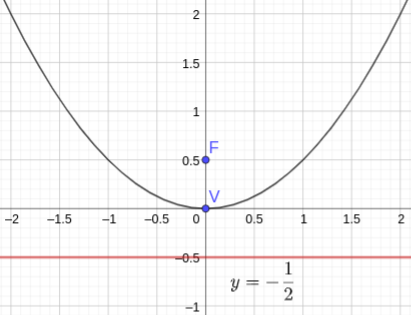
\includegraphics[width=0.5\textwidth]{cap_conicas/dados/fig_parabola_exer_x2_2y/fig}
\end{resp}

\begin{exer}
  Faça o esboço do gráfico da parábola de equação reduzida
  \begin{equation}
    x^2 = -2y.
  \end{equation}
  Identifique no esboço a reta diretriz, o foco e o vértice da parábola.
\end{exer}
\begin{resp}
  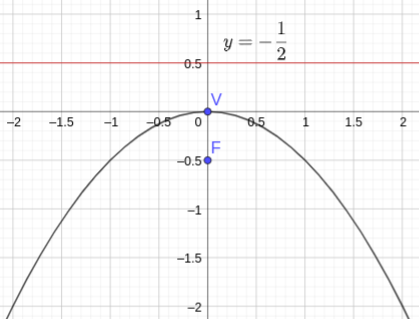
\includegraphics[width=0.5\textwidth]{cap_conicas/dados/fig_parabola_exer_x2-2y/fig}
\end{resp}

\begin{exer}
  Faça o esboço do gráfico da parábola de equação reduzida
  \begin{equation}
    y^2 = 2x.
  \end{equation}
  Identifique no esboço a reta diretriz, o foco e o vértice da parábola.
\end{exer}
\begin{resp}
  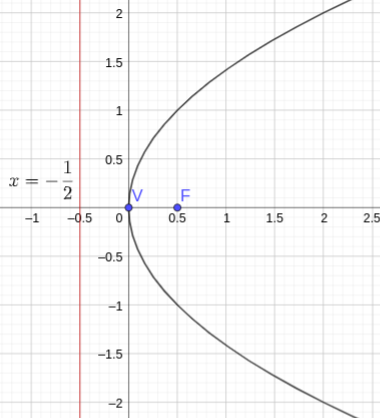
\includegraphics[width=0.5\textwidth]{cap_conicas/dados/fig_parabola_exer_y2_2x/fig}
\end{resp}

\begin{exer}
  Faça o esboço do gráfico da parábola de equação reduzida
  \begin{equation}
    y^2 = -2x.
  \end{equation}
  Identifique no esboço a reta diretriz, o foco e o vértice da parábola.
\end{exer}
\begin{resp}
  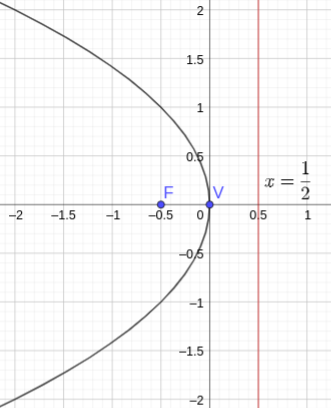
\includegraphics[width=0.5\textwidth]{cap_conicas/dados/fig_parabola_exer_y2-2x/fig}
\end{resp}

\begin{exer}
  Determine o foco de cada uma das seguintes parábolas:
  \begin{enumerate}[a)]
  \item $y = 2x^2$
  \item $y + 2x^2 = 0$
  \item $y^2 + 4x = 0$
  \item $\frac{1}{4}y^2 = x$
  \end{enumerate}
\end{exer}
\begin{resp}
  a)~$F=(0, \frac{1}{8})$; b)~$F=(0, -\frac{1}{8})$; c)~$F=(-1, 0)$; d)~$F=(1, 0)$
\end{resp}

%Este trabalho está licenciado sob a Licença Atribuição-CompartilhaIgual 4.0 Internacional Creative Commons. Para visualizar uma cópia desta licença, visite http://creativecommons.org/licenses/by-sa/4.0/deed.pt_BR ou mande uma carta para Creative Commons, PO Box 1866, Mountain View, CA 94042, USA.

\chapter{Superfícies Quádricas}\label{cap_superquad}
\thispagestyle{fancy}

Neste capítulo, fazemos um estudo introdutório sobre superífices quádricas.

\section{Introdução a superfícies quádricas}\label{cap_superquad_sec_intro}

Superfícies no espaço que podem ser descritas por equações da forma
\begin{equation}
  ax^2 + by^2 + cz^2 + 2dxy + 2exz + 2fyz + mx + ny + pz + q = 0
\end{equation}
são chamadas de \emph{superfícies quádricas}, sendo $a$, $b$, $c$, $d$, $e$, $f$, $m$, $n$, $p$ e $q$ coeficientes dados.

\subsection{Elipsoides}

Um \emph{elipsoide} centrado na origem é uma superfície quádrica de equação
\begin{equation}
  \frac{x^2}{a^2} + \frac{y^2}{b^2} + \frac{z^2}{c^2} = 1.
\end{equation}

\begin{ex}
  A Figura \ref{fig:sq_ex_elipsoide} é um esboço do gráfico da elipsoide de equação
  \begin{equation}\label{eq:sq_ex_elipsoide}
    \frac{x^2}{9} + \frac{y^2}{4} + z^2=1.
  \end{equation}
  
  \begin{figure}[H]
    \centering
    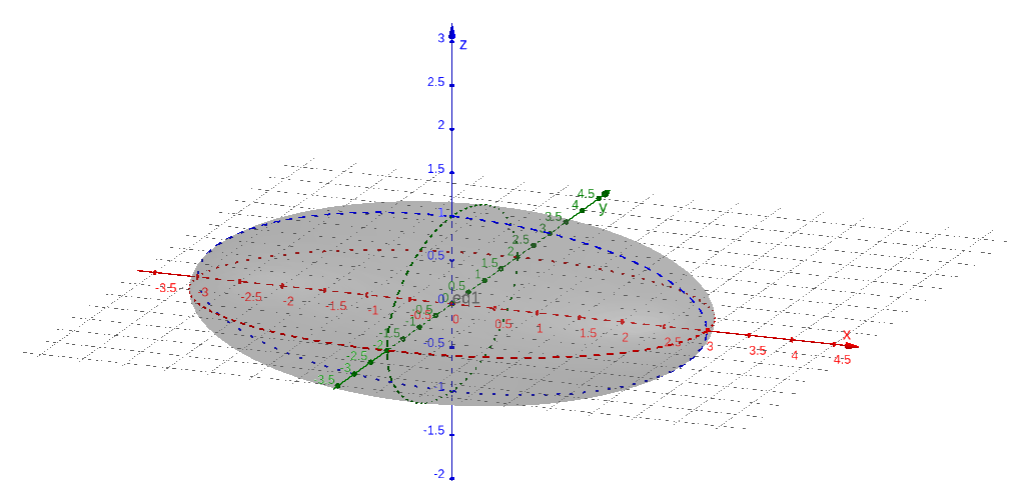
\includegraphics[width=\textwidth]{./cap_superquad/dados/fig_sq_ex_elipsoide/fig}
    \caption{Esboço do elipsoide de equação \eqref{eq:sq_ex_elipsoide}.}
    \label{fig:sq_ex_elipsoide}
  \end{figure}

  Observamos que a interseção deste elipsoide com o plano $X-Y$ (z=0) é a elipse de equação
  \begin{equation}
    \frac{x^2}{9}+\frac{y^2}{4}=1.
  \end{equation}
  Ou seja, é a elipse de vértice sobre o eixo maior $A_1=(-3,0)$ e $A_2=(3,0)$ e vértices sobre o eixo menor $B_1=(-2,0)$ e $B_2=(2,0)$.

  De forma análoga, temos que a interseção do elipsoide \eqref{eq:sq_ex_elipsoide} com o plano $X-Z$ ($y=0$) é a elipse de equação reduzida
  \begin{equation}
    \frac{x^2}{9} + z^2 = 1.
  \end{equation}
  Também, temos associada a elipse de equação reduzida
  \begin{equation}
    \frac{y^2}{4}+z^2=1
  \end{equation}
  que é obtida da interseção do elipsoide \eqref{eq:sq_ex_elipsoide} com o plano $Y-Z$ ($x=0$).  
\end{ex}

\subsection{Hiperboloides}

\subsubsection{Hiperboloides de uma folha}

Um hiperboloide de uma folha centrado na origem é uma superfície quádrica de equação
\begin{equation}
  \frac{x^2}{a^2}+\frac{y^2}{b^2}-\frac{z^2}{c^2}=1
\end{equation}
ou
\begin{equation}
  \frac{x^2}{a^2}-\frac{y^2}{b^2}+\frac{z^2}{c^2}=1
\end{equation}
ou
\begin{equation}
  -\frac{x^2}{a^2}+\frac{y^2}{b^2}+\frac{z^2}{c^2}=1
\end{equation}

\begin{ex}
  Vamos considerar o hiperboloide de equação
  \begin{equation}\label{eq:sq_ex_hiperboloide_z}
    \frac{x^2}{9}+\frac{y^2}{4}-z^2=1.
  \end{equation}
  Sua interseção com o plano $X-Y$ ($z=0$) é a elipse
  \begin{equation}
    \frac{x^2}{9}+\frac{y^2}{4}=1.
  \end{equation}
  Sua interseção com o plano $X-Z$ (y=0) é a hipérbole de equação reduzida
  \begin{equation}
    \frac{x^2}{9}-z^2=1.
  \end{equation}
  E, a interseção do hiperboloide com o plano $Y-Z$ ($x=0$) é a hipérbole de equação
  \begin{equation}
    \frac{y^2}{4}-z^2=1.
  \end{equation}
  
  A Figura \ref{fig:sq_ex_hiperboloide_z} é o esboço do gráfico do hiperboloide de equação \eqref{eq:sq_ex_hiperboloide_z}.

    \begin{figure}[H]
    \centering
    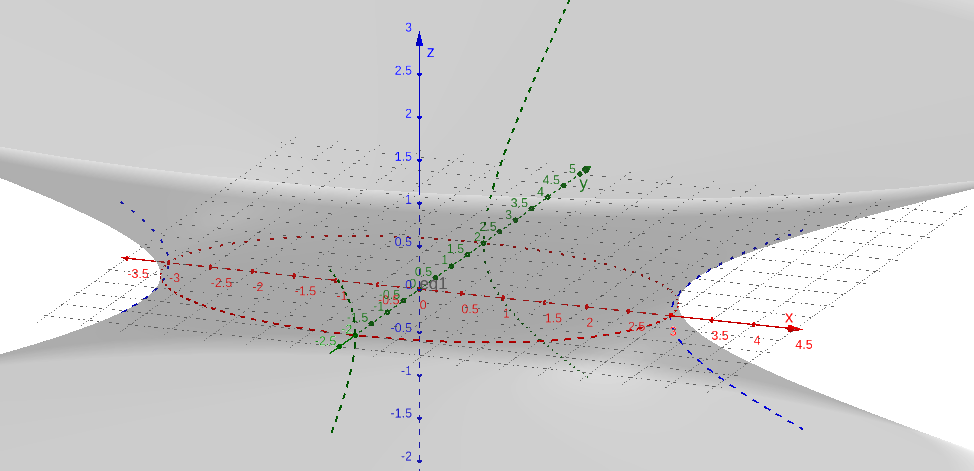
\includegraphics[width=\textwidth]{./cap_superquad/dados/fig_sq_ex_hiperboloide_z/fig}
    \caption{Esboço do hiperboloide de equação \eqref{eq:sq_ex_hiperboloide_z}.}
    \label{fig:sq_ex_hiperboloide_z}
  \end{figure}
\end{ex}

\begin{ex}
  A Figura \ref{fig:sq_ex_hiperboloide_x} é o esboço do gráfico do hiperboloide de equação
  \begin{equation}\label{eq:sq_ex_hiperboloide_x}
    -\frac{x^2}{9}+\frac{y^2}{4}+z^2=1.
  \end{equation}

  \begin{figure}[H]
    \centering
    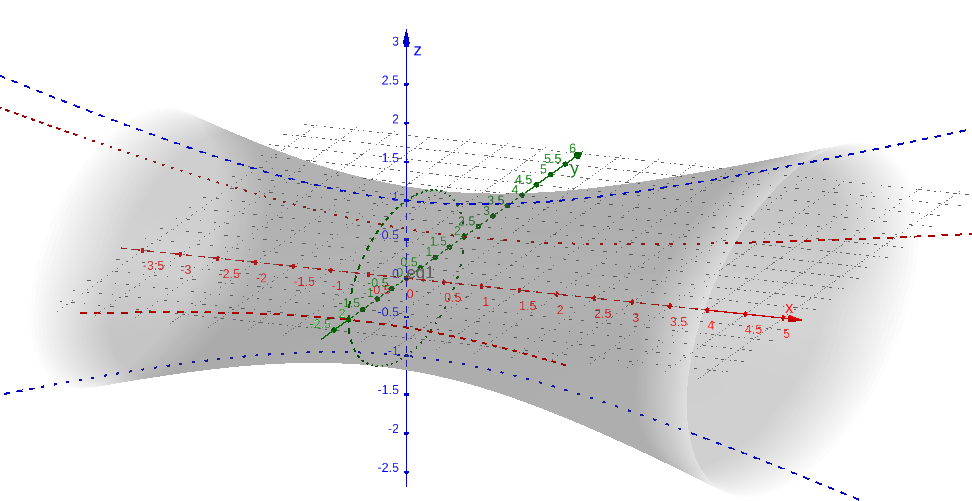
\includegraphics[width=\textwidth]{./cap_superquad/dados/fig_sq_ex_hiperboloide_x/fig}
    \caption{Esboço do hiperboloide de equação \eqref{eq:sq_ex_hiperboloide_x}.}
    \label{fig:sq_ex_hiperboloide_x}
  \end{figure}
  
  
  Sua interseção com o plano $X-Y$ ($z=0$) é a hipérbole
  \begin{equation}
    -\frac{x^2}{9}+\frac{y^2}{4}=1.
  \end{equation}
  Sua interseção com o plano $X-Z$ (y=0) é a hipérbole de equação reduzida
  \begin{equation}
    -\frac{x^2}{9}+z^2=1.
  \end{equation}
  E, a interseção do hiperboloide com o plano $Y-Z$ ($x=0$) é a elipse de equação
  \begin{equation}
    \frac{y^2}{4}+z^2=1.
  \end{equation}
\end{ex}

\subsubsection{Hiperboloides de duas folhas}

Hiperboloides de duas folhas têm equações
\begin{equation}
  \frac{x^2}{a^2}-\frac{y^2}{b^2}-\frac{z^2}{c^2}=1
\end{equation}
ou
\begin{equation}
  -\frac{x^2}{a^2}+\frac{y^2}{b^2}-\frac{z^2}{c^2}=1
\end{equation}
ou
\begin{equation}
  -\frac{x^2}{a^2}-\frac{y^2}{b^2}+\frac{z^2}{c^2}=1
\end{equation}

\begin{ex}
  Vamos considerar o hiperboloide de equação
  \begin{equation}\label{eq:sq_ex_hiperboloide_2f_x}
    \frac{x^2}{9}-\frac{y^2}{4}-z^2=1.
  \end{equation}
  Sua interseção com o plano $X-Y$ ($z=0$) é a hipérbole
  \begin{equation}
    \frac{x^2}{9}-\frac{y^2}{4}=1.
  \end{equation}
  Sua interseção com o plano $X-Z$ (y=0) é a hipérbole de equação reduzida
  \begin{equation}
    \frac{x^2}{9}-z^2=1.
  \end{equation}
  E, a interseção do hiperboloide com o plano $Y-Z$ ($x=0$) é vazia, pois não existem $y$ e $z$ que satisfazem a equação
  \begin{equation}
    -\frac{y^2}{4}-z^2=1,
  \end{equation}
  
    A Figura \ref{fig:sq_ex_hiperboloide_2f_x} é o esboço do gráfico do hiperboloide de equação \eqref{eq:sq_ex_hiperboloide_2f_x}.

    \begin{figure}[H]
    \centering
    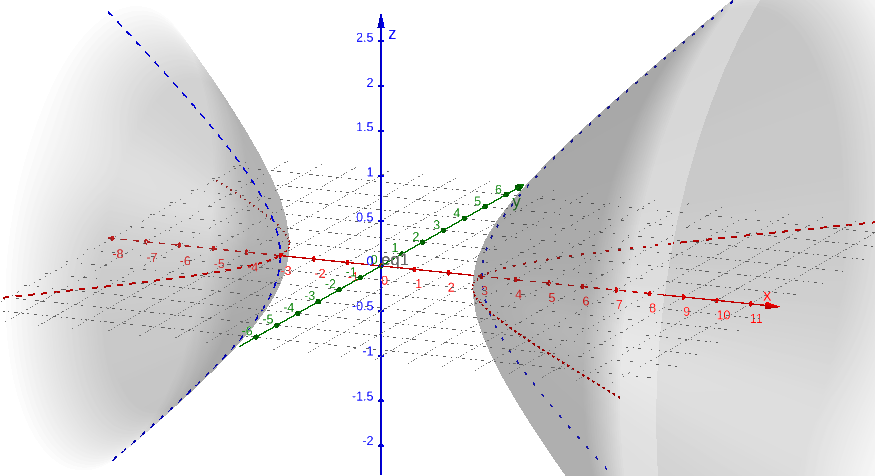
\includegraphics[width=\textwidth]{./cap_superquad/dados/fig_sq_ex_hiperboloide_2f_x/fig}
    \caption{Esboço do hiperboloide de equação \eqref{eq:sq_ex_hiperboloide_2f_x}.}
    \label{fig:sq_ex_hiperboloide_2f_x}
  \end{figure}
\end{ex}

\subsection{Paraboloide elíptico}

Um paraboloide elíptico tem equação
\begin{equation}
  \pm z = \frac{x^2}{a^2} + \frac{y^2}{b^2}
\end{equation}
ou
\begin{equation}
  \pm y = \frac{x^2}{a^2} + \frac{z^2}{c^2}
\end{equation}
ou
\begin{equation}
  \pm x = \frac{y^2}{b^2} + \frac{z^2}{c^2}
\end{equation}

\begin{ex}
  Vamos considerar o paraboloide elíptico de equação
  \begin{equation}\label{eq:sq_ex_parelip_z}
    z = \frac{x^2}{9}+\frac{y^2}{4}
  \end{equation}
  Não há valor $z<0$ que satisfaça a equação \eqref{eq:sq_ex_parelip_z}. Sua interseção com o plano $X-Y$ ($z=0$) é o ponto $(0, 0, 0)$. Agora, sua interseção com cada plano paralelo ao plano $X-Y$ e com $z=z_0>0$ é a elipse de equação
  \begin{equation}
    z_0 = \frac{x^2}{9}+\frac{y^2}{4}
  \end{equation}
  ou, equivalentemente,
  \begin{equation}
    \frac{x^2}{9z_0}+\frac{y^2}{4z_0}=1.
  \end{equation}

    A Figura \ref{fig:sq_ex_parelip_z} é o esboço do gráfico do paraboloide elíptico de equação \eqref{eq:sq_ex_parelip_z}.

    \begin{figure}[H]
    \centering
    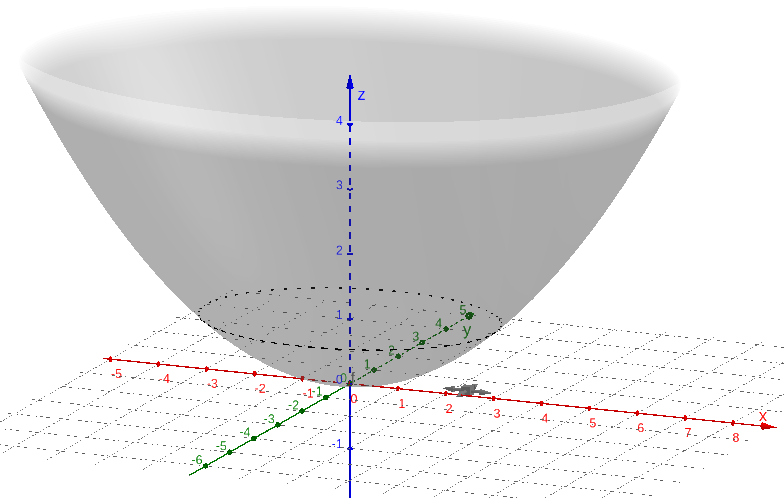
\includegraphics[width=\textwidth]{./cap_superquad/dados/fig_sq_ex_parelip_z/fig}
    \caption{Esboço do paraboloide elíptico de equação \eqref{eq:sq_ex_parelip_z}.}
    \label{fig:sq_ex_parelip_z}
  \end{figure}
\end{ex}

\begin{ex}
  O esboço do gráfico de paraboloide elíptico de equação
  \begin{equation}\label{eq:sq_ex_parelip-x}
    -x = \frac{y^2}{4}+z^2
  \end{equation}
  é dado na Figura \ref{fig:sq_ex_parelip-x}. Verifique!

    \begin{figure}[H]
    \centering
    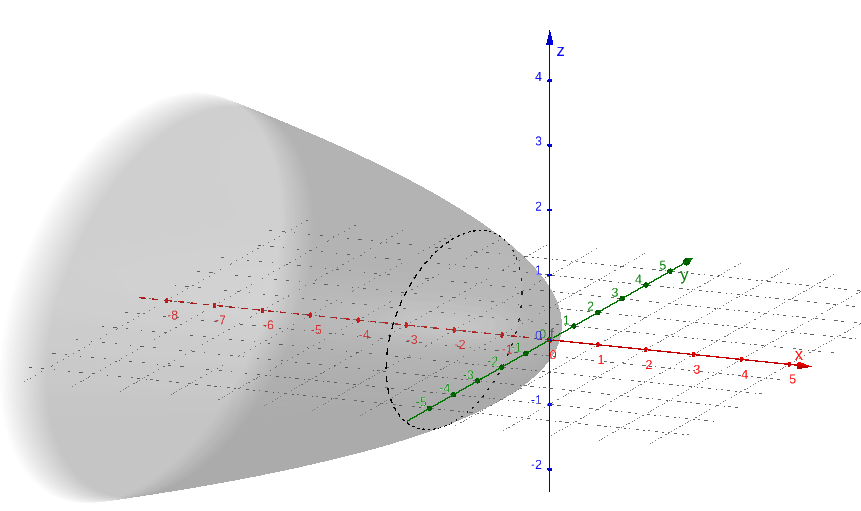
\includegraphics[width=\textwidth]{./cap_superquad/dados/fig_sq_ex_parelip-x/fig}
    \caption{Esboço do paraboloide elíptico de equação \eqref{eq:sq_ex_parelip-x}.}
    \label{fig:sq_ex_parelip-x}
  \end{figure}
\end{ex}

\subsection{Paraboloide hiperbólico}

Um paraboloide elíptico tem equação
\begin{equation}
  \pm z = \frac{x^2}{a^2} - \frac{y^2}{b^2}
\end{equation}
ou
\begin{equation}
  \pm y = \frac{x^2}{a^2} - \frac{z^2}{c^2}
\end{equation}
ou
\begin{equation}
  \pm x = \frac{y^2}{b^2} - \frac{z^2}{c^2}
\end{equation}

\begin{ex}
  Vamos considerar o paraboloide hiperbólico de equação
  \begin{equation}\label{eq:sq_ex_parhiper_z}
    z=\frac{x^2}{9}-\frac{y^2}{4}.
  \end{equation}
  Sua interseção com o plano $X-Y$ ($z=0$) são retas que satisfazem a equação
  \begin{equation}
    \frac{x^2}{9}-\frac{y^2}{4}=0.
  \end{equation}
  De fato, isolando $y$, obtemos as equações destas retas
  \begin{equation}
    y = \pm \frac{2}{3}x.
  \end{equation}
  Sua interseção com o plano $X-Z$ (y=0) é a parábola de equação
  \begin{equation}
    z=\frac{x^2}{9}.
  \end{equation}
  E, a interseção do paraboloide hiperbólico com o plano $Y-Z$ ($x=0$) é a parábola de equação
  \begin{equation}
    z=-\frac{y^2}{4}.
  \end{equation}
  
  A Figura \ref{fig:sq_ex_parhiper_z} é o esboço do gráfico do paraboloide hiperbólico de equação \eqref{eq:sq_ex_parhiper_z}.

    \begin{figure}[H]
    \centering
    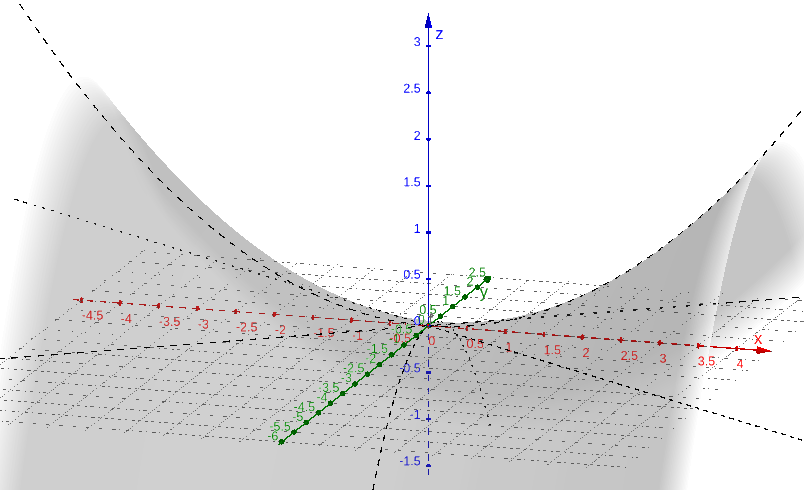
\includegraphics[width=\textwidth]{./cap_superquad/dados/fig_sq_ex_parhiper_z/fig}
    \caption{Esboço do paraboloide hiperbólico de equação \eqref{eq:sq_ex_parhiper_z}.}
    \label{fig:sq_ex_parhiper_z}
  \end{figure}
\end{ex}

\subsection*{Exercícios resolvidos}

\begin{exeresol}
  Escreva a equação do elipsoide que tem como interseções
  \begin{enumerate}[a)]
  \item com o plano $z=0$ a elipse
    \begin{equation}
      \frac{x^2}{4}+\frac{y^2}{16} = 1
    \end{equation}
  \item com o plano $y=0$ a elipse
    \begin{equation}
      \frac{x^2}{4}+\frac{z^2}{9} = 1
    \end{equation}
  \end{enumerate}
\end{exeresol}
\begin{resol}
  Um elipsoide tem equação
  \begin{equation}
    \frac{x^2}{a^2}+\frac{y^2}{b^2}+\frac{z^2}{c^2}=1.
  \end{equation}
  Sua interseção com o plano $X-Y$ ($z=0$) é a elipse de equação
  \begin{equation}
    \frac{x^2}{a^2}+\frac{y^2}{b^2}=1.
  \end{equation}
  Logo, do item a), temos $a^2=4$ e $b^2=16$.

  Agora, a interseção com o plano $X-Z$ ($y=0$) é a elipse de equação
  \begin{equation}
    \frac{x^2}{a^2}+\frac{z^2}{c^2}=1.
  \end{equation}
  Assim, do item b), obtemos $c^2=9$.

  Desta forma, concluímos que o elipsoide de equação
  \begin{equation}
    \frac{x^2}{4}+\frac{y^2}{16}+\frac{z^2}{9}=1.
  \end{equation}
\end{resol}

\begin{exeresol}
  Encontre a equação do paraboloide elíptico que contem a circunferência
  \begin{equation}
    x^2+z^2=1,\quad y=-2.
  \end{equation}
\end{exeresol}
\begin{resol}
  Para que o paraboloide contenha a circunferência
  \begin{equation}
    x^2+z^2=1,\quad y=-2,
  \end{equation}
  ele precisa abrir-se no sentido negativo na direção $y$. Logo, tem equação
  \begin{equation}
    -y = \frac{x^2}{a^2}+\frac{z^2}{b^2}.
  \end{equation}
  Fixado $y=-2$, a equação fica restrita a
  \begin{equation}
    2  = \frac{x^2}{a^2}+\frac{z^2}{b^2}.
  \end{equation}
  Notamos que para esta equação coincida com a circunferência $x^2+z^2=1$, devemos escolher $a^2=b^2=1/2$. Logo, concluímos que o paraboloide elíptico tem equação
  \begin{equation}
    -y = \frac{x^2}{\frac{1}{2}}+\frac{z^2}{\frac{1}{2}}.
  \end{equation}
\end{resol}

\subsection*{Exercícios}

\begin{exer}
  Classifique cada uma das seguintes superfícies quádricas:
  \begin{enumerate}[a)]
  \item $\displaystyle \frac{x^2}{2}-y^2+\frac{z^2}{4}=1$
  \item $\displaystyle x^2+\frac{y^2}{9}+\frac{z^2}{4}=1$
  \item $\displaystyle z = -x^2-\frac{y^2}{9}$
  \item $\displaystyle x^2 + y^2 + z^2 = 0$
  \end{enumerate}
\end{exer}
\begin{resp}
  a) hiperboloide de uma folha; b) elipsoide; c) paraboloide elíptico; d) ponto $(0, 0, 0)$
\end{resp}

\begin{exer}
  Forneça a equação do elipsoide que contem os pontos $P=(0,2,0)$, $Q=(-1,0,0)$ e $R=(0,0,1)$.
\end{exer}
\begin{resp}
  $\displaystyle x^2+\frac{y^2}{4}+z^2=1$
\end{resp}

\begin{exer}
  Forneça a equação do hiperboloide de duas folhas que tem interseções:
  \begin{enumerate}[a)]
  \item com o eixo $X-Y$ igual a hipérbole
    \begin{equation}
      -\frac{x^2}{16}+\frac{y^2}{4}=1
    \end{equation}
  \item com o eixo $Y-Z$ igual a hipérbole
    \begin{equation}
      \frac{y^2}{4}-\frac{z^2}{9}=1
    \end{equation}
  \end{enumerate}
\end{exer}
\begin{resp}
  $\displaystyle -\frac{x^2}{16}+\frac{y^2}{4}-\frac{z^2}{9}=1$
\end{resp}

\begin{exer}
  Forneça a equação do paraboloide elíptico que contem a elipse
  \begin{equation}
    \frac{x^2}{2}+z^2=1,\quad y=2.
  \end{equation}
\end{exer}
\begin{resp}
  $\displaystyle y = x^2+\frac{z^2}{\frac{1}{2}}$
\end{resp}

\begin{exer}
  Considere o hiperboloide de uma folha de equação
  \begin{equation}
    \frac{x^2}{9}-\frac{y^2}{4}+z^2=1.
  \end{equation}
  Classifique o lugar geométrico de sua interseção com cada um dos seguintes planos
  \begin{enumerate}
  \item $X-Y$
  \item $X-Z$
  \item $Y-Z$
  \end{enumerate}
\end{exer}
\begin{resp}
  a) hipérbole; b) elipse; c) hipérbole
\end{resp}


%resposta dos exercícios
\ifisbook
%Este trabalho está licenciado sob a Licença Atribuição-CompartilhaIgual 4.0 Internacional Creative Commons. Para visualizar uma cópia desta licença, visite http://creativecommons.org/licenses/by-sa/4.0/ ou mande uma carta para Creative Commons, PO Box 1866, Mountain View, CA 94042, USA.

\chapter*{Resposta dos Exercícios}\label{cap_respostas}
\addcontentsline{toc}{chapter}{Respostas dos Exercícios}

\shipoutAnswer
\fi

%references
\nocite{*}
\bibliographystyle{plain}
\bibliography{main}
\addcontentsline{toc}{chapter}{Referências Bibliográficas}

\ifisbook
\clearpage
\addcontentsline{toc}{chapter}{Índice Remissivo}
\printindex
\fi

\end{document}
